% ****** Start of file apssamp.tex ******
%
%   This file is part of the APS files in the REVTeX 4.1 distribution.
%   Version 4.1r of REVTeX, August 2010
%
%   Copyright (c) 2009, 2010 The American Physical Society.
%
%   See the REVTeX 4 README file for restrictions and more information.
%
% TeX'ing this file requires that you have AMS-LaTeX 2.0 installed
% as well as the rest of the prerequisites for REVTeX 4.1
%
% See the REVTeX 4 README file
% It also requires running BibTeX. The commands are as follows:
%
%  1)  latex aps25samp.tex
%  2)  bibtex apssamp
%  3)  latex apssamp.tex
%  4)  latex apssamp.tex
%
\documentclass[%
 reprint,
nofootinbib,
%superscriptaddress,
%groupedaddress,
%unsortedaddress,
%runinaddress,
%frontmatterverbose,
%preprint,
%showpacs,preprintnumbers,
%nofootinbib,
%nobibnotes,
%bibnotes,
aps,
%pra,
%prb,
%rmp,
%prstab,
%prstper,
%floatfix,
]{revtex4-1}

\usepackage[utf8]{inputenc}
\usepackage[english]{babel}
\usepackage{dsfont}
\usepackage{amsmath}
\usepackage{ mathrsfs }
\usepackage{amssymb}
\usepackage{graphicx}% Include figure files
\usepackage{dcolumn}% Align table columns on decimal point
\usepackage{bm}% bold math
\usepackage{amsmath}
\usepackage{varioref}
\usepackage{booktabs}
\usepackage[bottom]{footmisc}
\usepackage{minted} % for pseudocode

\usepackage{physics}
\usepackage[ruled,vlined]{algorithm2e}
\usepackage{algpseudocode}
\usepackage{listings}

\usepackage{booktabs}

\usepackage{tikz}
\usepackage{float}
\usepackage{siunitx}



\newcolumntype{C}{>{$}c<{$}}
\AtBeginDocument{
\heavyrulewidth=.08em
\lightrulewidth=.05em
\cmidrulewidth=.03em
\belowrulesep=.65ex
\belowbottomsep=0pt
\aboverulesep=.4ex
\abovetopsep=0pt
\cmidrulesep=\doublerulesep
\cmidrulekern=.5em
\defaultaddspace=.5em
}


\usepackage{hyperref}% add hypertext capabilities
%\usepackage[mathlines]{lineno}% Enable numbering of text and display math
%\linenumbers\relax % Commence numbering lines

%\usepackage[showframe,%Uncomment any one of the following lines to test
%%scale=0.7, marginratio={1:1, 2:3}, ignoreall,% default settings
%%text={7in,10in},centering,
%%margin=1.5in,
%%total={6.5in,8.75in}, top=1.2in, left=0.9in, includefoot,
%%height=10in,a5paper,hmargin={3cm,0.8in},
%]{geometry}

\renewcommand{\vec}[1]{\mathbf{#1}} %ny definisjon av \vec så det blir bold face i stedet for vector-pil.

\begin{document}


\title{Solving partial differential equations using finite difference schemes and studying temperature distribution in the lithosphere of western Norway}
\author{Fredrik Hoftun \& Mikkel Metzsch Jensen}

\affiliation{Department of Physics, University of Oslo\\}
\date{\today}



\begin{abstract}
In this two-part project we have solved the heat equation analytically and numerically, and used our numerical model to predict the temperature distribution in the lithosphere of western Norway given the presence of an radioactive enrichment from a subduction zone. In the first part of the project we successfully solved the heat equation analytically and numerically in one and two dimensions. We studied three numerical methods: The explicit forward Euler method, the implicit backwards Euler method and the implicit Crank-Nicolson method. We saw that explicit method is only numerically stable under the condition that $\Delta t \leq \frac{h^2}{2N}$ where $h$ is the constant spatial step-size for all dimensions $N$ and $\Delta t$ is a stable time-step. Both the implicit and Crank-Nicolson methods was found to be numerically stable for all values of $h$ and $\Delta t$. By investigating relative errors we found a qualitatively agreement with the theoretical statement of the error for the explicit and implicit method following $\mathcal{O}(\Delta t)$ and the Crank-Nicolson method following $\mathcal{O}(\Delta t^2)$. In addition we found a minimum error limit determined by the choice of spatial step length and time point of the solution. For the two-dimensional problem we only considered the explicit method but generally found a good agreement with the analytical solution.
\\
In the second part of the project we used the one dimensional explicit scheme to compute the steady state for the temperature distribution in the lithosphere without any radioactive enrichment. By using our obtained results for this base distribution we investigated the effects of an radioactive enrichment corresponding to the effects of a subduction zone under Norway one billion years ago. We found the predicted present difference to be 14.31 $^{\circ}$C at a depth of 66 km. For more reachable depths in the interval [1.0, 12.1] km we found the difference to be in the range [0.3, 3.3] $^{\circ}$ C. If this were to be verified by real life measurements this would serve as supporting evidence for the subduction taking place as proposed by the geologist.



\end{abstract}

\vfill
\onecolumngrid
\footnotesize{{Link to our GitHub repository: \url{https://github.com/mikkelme/project5_FYS3150}}}
\twocolumngrid
\maketitle
\newpage


\section{Introduction}
The partial differential equation is an important type of equation which appears in many mathematically-oriented scientific fields, such as physics and engineering. For instance, it is used in relation to heat, sound, diffusion, electrostatics, electrodynamics, fluid dynamics, elasticity, general relativity and quantum mechanics \cite{wiki:PDE}. In this article we shall study the heat equation. For the first part we are going to take a mathematical approach to the dimensionless version of the heat equation. We are going to solve it both analytically and numerically in one and two dimensions. For the numerical solution, we study three different methods: The explicit forward Euler method, the implicit backwards Euler method and the Crank-Nicolson method. The forward Euler method is based on the forward Euler scheme for ordinary differential equations (ODE), likewise the backward Euler method is based on backwards ODE-method. The Crank-Nicolson method is a combination of the two earlier methods. By comparing analytical and numerical result we discuss the pros and cons of the mentioned methods. \\
\\
For the second part we will use our findings to study the temperature distribution in the lithosphere. The lithosphere describes the outer layer of the earth till a depth of approximately 12 km. Geologists have proposed that there was an active subduction zone on the western coast of Norway about one billion years ago (see illustration on figure \ref{fig:geo_fig}. When subducting, the oceanic lithosphere melts and releases water and other chemical components. Most of them go to the surface but some of them may be trapped in the mantle wedge (bottom sublayer of the lithosphere) above the subducting slab. This process is called the refertilization of the mantle and since the new chemical components contain more radioactive elements, we expect the heat production in the mantle to increase. With the use of data from the Department of Geoscience at the University of Oslo (GUiO) we can use our numerical models to calculate the thermal evolution of the lithosphere given the assumption of a radioactive enrichment one billion years ago. By that we can estimate how such an event will propagate into today's measurements of the temperature distribution, and whether we should be able to measure the effects of such an event at present time.
\begin{figure}[H]
    \centering
    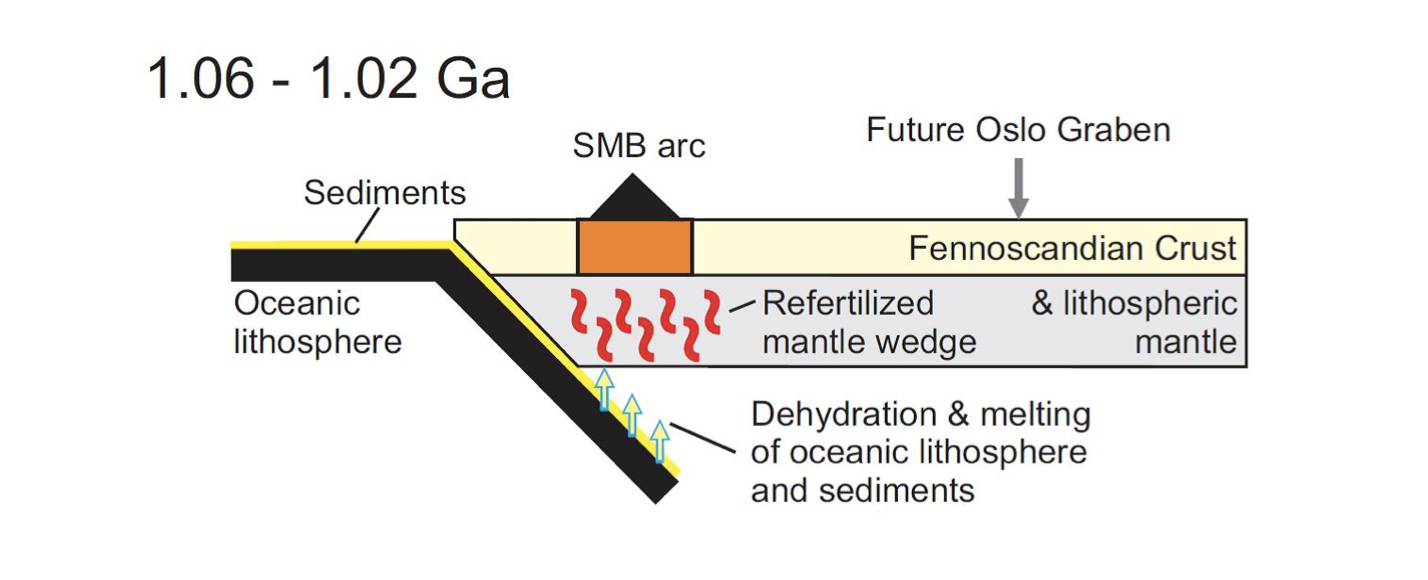
\includegraphics[width=0.5\textwidth]{figures/geo_fig.png}
    \caption{The figure shows the geological system which we are going to model. Note that we divide the Fennoscandian Crust in the upper and lower crust later on. The enrichment of the mantle comes from the subduction of the oceanic lithosphere from the left in the picture. The figure is taken from the project description PDF.\cite{project_description}}
    \label{fig:geo_fig}
\end{figure}

\section{Method}
\subsection{Defining the problem - Heat equation in 1D} \label{sec:defproblem1D}
For the first part we are going to address the dimensionless general version of the one dimensional heat equation given as
\begin{equation}
    \frac{\partial^2 u(x,t)}{\partial x^2} = \frac{\partial u(x,t)}{\partial t}, \qquad t>0 \quad x \in [0,L]
    \label{eq:num_HQ}
\end{equation}
where $x$ is the spatial coordinate, $t$ is time and $L$ is the length of the x-region of interest. We are going to use the initial conditions
\begin{align*}
    u(x,0) = 0, \qquad 0<x<L
\end{align*}
and boundary conditions
\begin{align*}
    u(0,t) &= 0, \qquad t \ge 0 \\
    u(L,t) &= 1, \qquad t \ge 0
\end{align*}
In order to solve the problem efficiently when using numerical methods we introduce a modified solution $v(x,t)$:
\begin{align*}
    v(x,t) = u(x,t) + f(x)
\end{align*}
for which we demand the simplified boundary conditions to be
\begin{align*}
     v(0,t) = v(L,t) = 0, \quad t\ge0
\end{align*}
We must then determine the function $f(x)$, describing the steady state, such that these boundary criteria are met. We use that $v(x,t)$ must obey the diffusion equation which yields
\begin{align*}
    \frac{\partial^2u}{\partial x^2} + \frac{d^2f}{dx^2} - \frac{\partial u}{\partial t} = 0
\end{align*}
Since we also can assume $u(x,t)$ to obey the diffusion equation we get
\begin{align*}
     \frac{d^2f}{dx^2} = 0 \quad \Longrightarrow \quad  f(x) = ax + b
\end{align*}
By using the required conditions $f(0) = 0$ and $f(L) = -1$ we find the linear solution:
\begin{align*}
    f(x) = -\frac{1}{L}x
\end{align*}
We will solve the problem numerically for $v(x,t)$ and transform back to the actual solution $u(x,t)$ by simply subtracting the function $f(x)$.
\subsubsection{Discretizing the problem}
In order to solve the problem numerically we make a discretization. We introduce different step lengths $\Delta t$ for time and
\begin{align*}
    \Delta x = \frac{L}{n+1}
\end{align*}
for x, where we have discretized the variables as
\begin{align*}
    x_i &= i\Delta x, \qquad 0 \le i \le n+1 \\
    t_j &= j\Delta t, \qquad j \ge 0
\end{align*}


\subsection{Explicit Forward Euler}
The explicit scheme is derived by the use of standard approximations for the derivatives. With the forward and second-order central approximation we obtain:
\begin{align*}
    v_t = \frac{\partial v(x,t)}{\partial t} &= \frac{v(x,t + \Delta t) - v(x,t)}{\Delta t} + \mathcal{O}(\Delta t)  \\
     v_{xx} = \frac{\partial^2 v(x,t)}{\partial x^2} &= \frac{v(x + \Delta x, t) - 2v(x,t) + v(x -\Delta x, t)}{\Delta x^2} + \mathcal{O}(\Delta x^2)
\end{align*}
For the discretized case we use the notation:
\begin{align*}
   v_t &\approx \frac{v_{ij+1} - v_{ij}}{\Delta t} \\
   v_{xx} &\approx \frac{v_{i+1j} - 2v_{ij} + v_{i-1j}}{\Delta x^2}
\end{align*}
We insert this into the one-dimensional diffusion equation and obtain:
\begin{align*}
    \frac{v_{ij+1} - v_{ij}}{\Delta t} = \frac{v_{i+1j} - 2v_{ij} + v_{i-1j}}{\Delta x^2}
\end{align*}
By defining $\alpha = \Delta t/\Delta x^2$ we can rewrite the above equation and arrive at the explicit scheme:
\begin{equation}
    v_{ij+1} = \alpha v_{i-1j} + (1-2\alpha)v_{ij} + \alpha v_{i+1j}
    \label{eq:explicit}
\end{equation}
Here $v_{ij+1}$ is the only unknown quantity which are explicit defined by the right hand side of equation \ref{eq:explicit} which is known. From the derivation approximations we find that the truncation error is $\mathcal{O}(\Delta x^2)$ and $\mathcal{O}(\Delta t)$. For the purpose of investigating the stability condition we can reformulate the explicit scheme \ref{eq:explicit} as a matrix equation $$V_{j+1} = \textbf{A} V_j$$ where
\begin{equation}
    \vec{A} = \begin{bmatrix}
                    1-2\alpha & \alpha & 0 & 0 & \cdots \\
                    \alpha & 1-2\alpha & \alpha & 0 & \cdots \\
                    \cdots & \cdots & \cdots & \cdots & \cdots \\
                    \cdots & \cdots & \cdots & \cdots & \alpha \\
                    0 & 0 & \cdots & \alpha & 1-2\alpha
    \end{bmatrix}
     , \qquad V_j =  \begin{bmatrix}
                        v_{1j} \\
                        v_{2j} \\
                        \vdots \\
                        v_{nj} \\
                    \end{bmatrix}
    \label{eq:A_Ex}
\end{equation}

\subsubsection{Stability criteria} \label{sec:exstab}
The explicit method is quite straight forward and easy to implement, but it has a rather weak stability condition given by
\begin{align*}
    \alpha = \frac{\Delta t}{\Delta x^2} \le \frac{1}{2}
\end{align*}
The stability condition is derived by finding the conditions for which the solution converges to a certain value.
% This will happen according to our initial conditions in section \ref{sec:defproblem1D}.
The method will converge if the spectral radius $\rho(\textbf{A})$ of a matrix $\textbf{A}$ satisfies the condition
\begin{align} \label{eq:specrad}
    \rho(\textbf{A}) < 1
\end{align}
where the spectral radius is defined as
\begin{align*}
  \rho(A) = \text{max}\{|\lambda|:\det (\textbf{A}-\lambda \hat I) = 0\}
\end{align*}
This can be interpreted as the smallest number such that a circle with radius centered at zero in the complex plane contains all eigenvalues of $\textbf{A}$. If the matrix is positive definite, the condition in equation \ref{eq:specrad} is always satisfied. The matrix $\textbf{A}$ from the rewritten explicit scheme (see \ref{eq:A_Ex}) can be rewritten as $$\textbf{A} = \hat I - \alpha \hat B$$ where $\hat{I}$ is the identity matrix and
\begin{align*}
    \hat{\vec{B}} = \begin{bmatrix}
                    2 & -1 & 0 & 0 & \cdots \\
                    -1 & 2 & -1 & 0 & \cdots \\
                    \cdots & \cdots & \cdots & \cdots & \cdots \\
                    \cdots & \cdots & \cdots & \cdots & -1 \\
                    0 & 0 & \cdots & -1 & 2
    \end{bmatrix}
\end{align*}
with eigenvalues $\mu_i$. This gives us the following eigenvalues for \textbf{A}: $$\lambda_i = 1-\alpha \mu_i$$
We see that the elements of $\hat{\vec{B}}$ are $$b_{ij} = 2 \delta_{ij} - \delta_{i-1j} - \delta_{i+1j}$$ which we can use to set up a set of eigenequations $$(\hat{\vec{B}} \hat x)_i = \mu_i x_i$$ or more explicitly
\begin{align}
    (\hat{\vec{B}} \hat x)_i &= \sum_{j=1}^n (2 \delta_{ij} - \delta_{i-1j} - \delta_{i+1j})x_j \nonumber \\
    &= 2x_i -x_{i-1} - x{i+1} = \mu_i x_i
    \label{eq:stab_eigeq}
\end{align}
Since model has zeroes at its boundaries, like the $\sin n \pi$ function, we assume that we can perform a basis shift from x to a sine
\begin{align*}
    x = (\sin \theta, \sin 2\theta, ..., \sin n\theta ), \qquad \theta = \frac{L \pi}{n+1}
\end{align*}
We insert this into equation \ref{eq:stab_eigeq} and get $$2 \sin (i\theta)-\sin((i-1)\theta)-\sin((i+1)\theta) = \mu_i \sin(i\theta)$$ which can be rewritten as $$2(1-\cos(\theta))\sin(i\theta) = \mu_i \sin(i\theta)$$ We can now swap back to the x basis and have our final equation $$2(1-\cos(\theta))x_i= \mu_i x_i$$ with eigenvalues $$\mu_i = 2(1-\cos \theta)$$ We can now use the condition in equation \ref{eq:specrad} and see that
\begin{align*}
    -1 &< \lambda_i < 1\\
    -1 &< 1-\alpha 2(1-\cos \theta) < 1\\
    \to \alpha &< (1-\cos \theta)^{-1}
\end{align*}
We see that the condition is satisfied for $$\alpha = \frac{\Delta t}{\Delta x^2} \le \frac{1}{2}$$ and the derivation is finished.\cite{pdepdf}

\subsubsection{Implementation}
The explicit scheme is very simple to implement. In a time loop over the position index, we use the explicit scheme \ref{eq:explicit} to compute the new solution vector $v_{new}$ from the present solution vector $v$. The practical implantation can be done as shown in the following example of code:
\begin{minted}[breaklines, breakautoindent = true]{cpp}
for (int tstep = 1; tstep <= timesteps){
    for (int i = 1; i < N+1; i++){
    	v_new[i] = alpha*v[i-1] + (1-2*alpha)*v[i]+alpha*v[i+1];
    }
    v = v_new;
}
\end{minted}
Note that the inner loop does not include the boundary.

\subsection{Implicit Backwards Euler}
For the derivation of the implicit scheme we use a similar approach as for the explicit scheme. However, instead of using the forward formula for the first derivative $v_t$ we use the backwards formula:
\begin{align*}
     v_t = \frac{\partial v(x,t)}{\partial t} &\approx \frac{v(x,t) - v(x,t - \Delta t)}{\Delta t} + \mathcal{O}(\Delta t)
\end{align*}
For the second derivative $v_{xx}$ we stick to the second-order central approximation.
% \begin{align*}
%     v_{xx} = \frac{\partial^2 v(x,t)}{\partial x^2} &\approx \frac{(x + \Delta x, t) - 2v(x,t) + v(x-\Delta x,t)}{\Delta x^2}
% \end{align*}
We define again $\alpha = \Delta t/\Delta x^2$ and obtain the implicit scheme
\begin{align*}
    \frac{v_{ij} - v_{ij-1}}{\Delta t} = \frac{v_{i+1j} -2v_{ij} + v_{i-1j}}{\Delta x^2}
\end{align*}
$\quad \Longleftrightarrow$
\begin{equation}
    v_{ij-1} = -\alpha v_{i-1j} + (1+2\alpha)v_{ij} - \alpha v_{i+1j}
    \label{eq:implicit}
\end{equation}
where $v_{ij-1}$ is the only unknown quantity. Since we have the boundary conditions $v_{0,t} = v_{L,t} = 0$ we can reformulate the algorithm with a matrix-vector formulation
\begin{align}\label{eq:Immatrix}
    \vec{A}V_j = V_{j-1}
\end{align}
where
\begin{align}
    \vec{A} = \begin{bmatrix}
                    1+2\alpha & -\alpha & 0 & 0 & \cdots \\
                    -\alpha & 1+2\alpha & -\alpha & 0 & \cdots \\
                    \cdots & \cdots & \cdots & \cdots & \cdots \\
                    \cdots & \cdots & \cdots & \cdots & -\alpha \\
                    0 & 0 & \cdots & -\alpha & 1+2\alpha
    \end{bmatrix}
     , \qquad V_j =  \begin{bmatrix}
                        v_{1j} \\
                        v_{2j} \\
                        \vdots \\
                        v_{nj} \\
                    \end{bmatrix}
    \label{eq:A_Im}
\end{align}
This is a tridiagonal matrix which can be solved with the use of the Thomas algorithm. Since this matrix is diagonally dominant we know that the Thomas algorithm is stable. We used this in an earlier project and will reuse the code (see \cite{project1}). Since we used similar derivation approximations we find that the truncation error is also $\mathcal{O}(\Delta x^2)$ and $\mathcal{O}(\Delta t)$, similar to the explicit scheme.

\subsubsection{Stability criteria}
Unlike the explicit scheme the implicit scheme is stable for all values of $\Delta t$ and $\Delta x$. We can show this from equation \ref{eq:implicit} and the matrix \textbf{A} (\ref{eq:A_Im}) by rewriting it into a similar form as we did in section \ref{sec:exstab}. This yields $${\vec{A}} = \hat I + \alpha \hat{\vec{B}}$$ with eigenvalues $$\lambda_i = 1 + \alpha 2 (1-\cos \theta) > 1$$ This results in $$\rho(\textbf{A})>1$$ However in the implicit scheme we use the Thomas algorithm and iterate over the inverse of \textbf{A} with spectral radius $\rho(\textbf{A}^{-1})<1$ satisfying the condition of equation \ref{eq:specrad} and making the implicit scheme stable for any values of $\Delta x$ and $\Delta t$.

\subsubsection{Implementation}
In order to implement the implicit scheme we need to construct a vector for the diagonal $a$ and for the off-diagonals $b,c$. We then simply loop over a function that calls the tridiagonal solver performing a forward- and backward substitution on the matrix and updating the solution vector $v$. This can be done as sketched in the following code:
\begin{minted}[breaklines, breakautoindent = true]{cpp}
for (int i = 0; i < N+2; i++){
	    a[i] = c[i] = -alpha;
	    b[i] = 1+2*alpha;
}
for (int tstep = 1; tstep <= timesteps){
    tridag(N, a, b, c, v, v_new);
    v = v_new;
}
\end{minted}

% For a singe time-step do:
% \begin{itemize}
%     \item Initialize the tridiagonal matrix with all the values.
%     \item Compute the Thomas algorithm by first "forward substituting" and then "backward substituting" to get $v_{ij+1}$.
% \end{itemize}
% This can be done for all time-steps.


\subsection{Crank-Nicolson scheme}
For the last method we combine the explicit and implicit scheme. We introduce the parameter $\theta$  (the so-called $\theta$-rule) and set up the following equation.
\begin{align*}
    \frac{\theta}{\Delta x^2} (v_{i+1j} -2v_{ij} + v_{i-1j}) + \frac{1 - \theta}{\Delta x^2}(v_{i+1j-1} - 2v_{ij-1} + v_{i-1j-1}) \\ = \frac{1}{\Delta t}(v_{ij} - v_{ij-1})
\end{align*}
This is a combination of the explicit and scheme which is weighted by the variable $\theta$. By choosing $\theta = 0$ we get the forward formula and thereby the explicit scheme. $\theta = 1$ yields the backwards formula and thereby the implicit scheme. By choosing $\theta = 1/2$ we get an equal combination which is the Crank-Nicolson scheme:
\begin{align*}
    \frac{v_{i+1j} -2v_{ij} + v_{i-1j} + v_{i+1j-1} - 2v_{ij-1} + v_{i-1j-1} }{2\Delta x^2} = \frac{v_{ij} - v_{ij-1}}{\Delta t}
\end{align*}
By using the same definition $\alpha = \Delta t/\Delta x^2$ we can rewrite the scheme as
\begin{multline}\label{eq:CN}
 -\alpha v_{i+1j} + (2+2\alpha)v_{ij} - \alpha v_{i-1j} \\
    = \alpha v_{i+1j-1} + (2-2\alpha)v_{ij-1} + \alpha v_{i-1j-1}
\end{multline}

or with a matrix-vector formulation as
\begin{align}\label{eq:CNmatrix}
    (2{\hat{\vec{I}}} + \alpha {\hat{\vec{B}}})V_j = (2\hat{I} - \alpha \hat{\vec{B}})V_{j-1}
\end{align}
where
\begin{align*}
    \hat{\vec{B}} = \begin{bmatrix}
                    2 & -1 & 0 & 0 & \cdots \\
                    -1 & 2 & -1 & 0 & \cdots \\
                    \cdots & \cdots & \cdots & \cdots & \cdots \\
                    \cdots & \cdots & \cdots & \cdots & -1 \\
                    0 & 0 & \cdots & -1 & 2
    \end{bmatrix}
     , \qquad V_j =  \begin{bmatrix}
                        v_{1j} \\
                        v_{2j} \\
                        \vdots \\
                        v_{nj} \\
                    \end{bmatrix}
\end{align*}
It can be showed that the truncation error for this scheme is $\mathcal{O}(\Delta x^2)$ and $\mathcal{O}(\Delta t^2)$.

\subsubsection{Stability criteria}
Like the implicit scheme the CN scheme is stable for all values of $\Delta x$ and $\Delta t$. We can make a similar argument as we did for the implicit scheme by applying the Thomas algorithm on equation \ref{eq:CNmatrix}. We rewrite equation \ref{eq:CNmatrix} on the form $$(2{\hat{\vec{I}}} + \alpha {\hat{\vec{B}}})V_j = W_{j-1} , \qquad W_{j-1} = (2\hat{I} - \alpha \hat{\vec{B}})V_{j-1}$$
where ${W_{j-i}}$ is known. We see that we have an equation on a similar form to equation \ref{eq:Immatrix} for the implicit scheme with eigenvalues that are always larger than one. Since $$\rho(2{\hat{\vec{I}}} + \alpha {\hat{\vec{B}}})>1$$ and we use the inverse in the Thomas algorithm we arrive at the result, similar to the implicit scheme, that the solution is stable for all values of $\Delta x$ and $\Delta t$.


\subsubsection{Implementation}
The CN scheme is a combination of the explicit and implicit schemes. In a time loop we compute the right hand side of equation \ref{eq:CN} for the Crank-Nicolson scheme with the previous time-step values and use the Thomas algorithm (tridiagonal solver) to compute the values at the next time-step. This can be done as showed in the following code example:
\begin{minted}[breaklines, breakautoindent = true]{cpp}
for (int i = 0; i < N+2; i++){
	a[i] = c[i] = -alpha;
	b[i] = 2+2*alpha;
}
for (int tstep = 1; tstep <= timesteps){
	for (int i = 1; i < N+1; i++){
		v_old[i] = alpha*v[i-1] + (2-2*alpha)*v[i]+alpha*v[i+1];
	}
	tridag(N, a, b, c, v_old, v);
}
\end{minted}
% For a single time-step do:
% \begin{itemize}
%     \item Initialize the tridiagonal matrix with all the values.
%     \item Use the right hand side of equation \ref{eq:CN} with the previous time-step values and use the Thomas algorithm to compute the values at the next time-step.
% \end{itemize}
% This can be done for all-timesteps.

\subsection{Analytic solution the the diffusion equation}
For the purpose of having something to compare our numerical results against we can derive an analytical solution to the diffusion equation. We assume that the solution can be found with separation of variables
\begin{align*}
    v(x,t) = F(x)G(t)
\end{align*}
By inserting this into the diffusion equation we find
\begin{align*}
    \frac{F''(x)}{F(x)} = \frac{G'(t)}{G(t)}
\end{align*}
We see that both sides of the equation must be equal to a constant which we define as $-\lambda^2$. This gives the equations:
\begin{align*}
    &F''(x) + \lambda^2F(x) = 0& &G'(t) = -\lambda^2 G(t)&
\end{align*}
with general solutions
\begin{align*}
    &F(x) = A\sin{(\lambda x)} + B\cos{(\lambda x)}& &G(t) = Ce^{-\lambda^2t}&
\end{align*}
By the use of the boundary conditions for $v(x,t)$, which translates to $F(0) = F(L) = 0$, we get $B = 0$ and $\lambda = n\pi/L$ where $n = 1,2,3, \hdots$ is a natural number. The solution is then given as
\begin{align}
    v(x,t) = A_n \sin{(\frac{n\pi x}{L})}e^{-\frac{n^2\pi^2t}{L^2}}
\end{align}
Since there are infinitely many possible values for $n$ we have infinitely many solutions. Because the diffusion equation is linear we know that a superposition of solutions is also a solution. Therefore we can write
\begin{align*}
    v(x,t) = \sum_{n=1}^\infty A_n \sin{(\frac{n\pi x}{L})}e^{-\frac{n^2\pi^2t}{L^2}}
\end{align*}
The coefficient $A_n$ can be found from the initial condition. Since $u(x,0) = 0$ we have
\begin{align*}
    v(x,0) = f(x) =  \sum_{n=1}^\infty A_n \sin{(\frac{n\pi x}{L})}
\end{align*}
We recognize that $A_n$ is the Fourier coefficients for the functions $f(x)$ and it is given from the theory of Fourier series that
\begin{align*}
    A_n = \frac{2}{L}\int_0^L f(x) \sin{(\frac{n\pi x}{L})} dx
\end{align*}
By using integration by parts we can solve the integral and get
\begin{align*}
    A_n = 2\frac{ n\pi \cos{(n\pi)} - \sin{(n\pi)}}{n^2\pi^2} = \frac{2\cos{(n\pi)} }{n\pi}
\end{align*}
This gives the final solution
\begin{equation}
    v(x,t) = \sum_{n=1}^\infty  \frac{2\cos{(n\pi)} }{n\pi} \sin{(\frac{n\pi x}{L})}e^{-\frac{n^2\pi^2t}{L^2}}
    \label{eq:1D_ana}
\end{equation}

\subsection{Moving to two dimensions}\label{sec:2D}
In order to study a wider variety of systems we will often benefit from adding an extra dimension. We will expand our system to $2+1$ dimensions meaning 2 spatial dimensions $x$ and $y$ and one time dimension $t$. The heat equation then becomes
\begin{align}
    \frac{\partial^2 u(x,y,t)}{\partial x^2} + \frac{\partial^2 u(x,y,t)}{\partial y^2} = \frac{\partial u(x,t)}{\partial t}, \quad t>0 \quad x,y \in [0,L]
    \label{eq:2D_HQ}
\end{align}
For simplicity we choose the simplest possible boundary conditions of having all sides fixed to zero.
\begin{align*}
      u(0,y,t) &= u(L,y,t) = 0 \\
      u(x,0,t) &= u(x, L, t) = 0
\end{align*}
For the initial condition we choose the following function, also for the sake of simplicity:
\begin{align*}
     u(x,y,0) &= \sin{(\frac{\pi x}{L})} \sin{(\frac{\pi y}{L})}, \qquad x,y \in (0,L) \\
\end{align*}
We assume to have a $L\times L$ lattice with equally many mesh points $n+2$ in both x- and y-direction. This gives the positional step length $h = L/(n+1)$, and we discretize the variables as
\begin{align*}
    &x_i = ih&  &0 \le i \le n+1& \\
    &y_j = jh&  &0 \le j \le n+1& \\
    &t_l = l\Delta t& &l \ge 0&
\end{align*}

\subsubsection{Explicit scheme for the 2D problem}
The simplest solution to the two dimensional problem is found by the use of the explicit scheme. We use again the the second-order central approximation for the positional derivative which yields
\begin{align*}
     u_{xx} &= \frac{u(x + h,y, t) - 2u(x,y,t) + u(x -h,y,t)}{h^2} + \mathcal{O}(h^2) \\
     u_{yy} &= \frac{u(x,y+h, t) - 2u(x,y,t) + u(x,y-h,t)}{h^2} + \mathcal{O}(h^2)
\end{align*}
With discretized notation we now rewrite this as
\begin{align*}
    u_{xx} &= \frac{u_{i+1j}^l - 2u_{ij}^l + u_{i-1j}^l}{h^2} + \mathcal{O}(h^2)\\
    u_{yy} &=  \frac{u_{ij+1}^l - 2u_{ij}^l + u_{ij-1}^l}{h^2} + \mathcal{O}(h^2)
\end{align*}
For the time derivative we use the forward Euler formula which we can write in the discretized form as
\begin{align*}
    u_t = \frac{u_{ij}^{l+1} + u_{ij}^l}{\Delta t} + \mathcal{O}(\Delta t)
\end{align*}
We insert this into the two-dimensional heat equation \ref{eq:2D_HQ} and get
\begin{align*}
    \frac{u_{i+1j}^l - 2u_{ij}^l + u_{i-1j}^l}{h^2} + \frac{u_{ij+1}^l - 2u_{ij}^l + u_{ij-1}^l}{h^2} = \frac{u_{ij}^{l+1} + u_{ij}^l}{\Delta t}
\end{align*}
By reusing the definition $\alpha = \Delta t / \Delta h^2$ we find the final scheme to be
\begin{align} \label{eq:2D_explicit}
    u_{ij}^{l+1} = u_{ij}^l + \alpha(u_{i+1j}^l + u_{i-1j}^l + u_{ij+1}^l + u_{ij-1}^l -4v_{ij}^l)
\end{align}
Again the left hand side is the only unknown term which determine the solution at the next time step. Since we start at $t = t_0$ the solution is entirely determined by the boundary and initial conditions. We can use a similar approach for the implementation of this as used for the one dimensional problem.

\subsubsection{Stability criteria}
We found the stability criteria for the 1D explicit scheme in section \ref{sec:exstab} given by \begin{align*}
    \alpha = \frac{\Delta t}{\Delta x^2} \le \frac{1}{2}
\end{align*}
By extending our scheme to two dimensions we get the new stability criteria
\begin{align*}
    \frac{\Delta t}{\Delta x^2} + \frac{\Delta t}{\Delta y^2} \le \frac{1}{2}
\end{align*}
For $\Delta x  =\Delta y = h$ we see that we get a new stability criteria
\begin{align*}
    \Delta t &\le \frac{1}{2} \left( \frac{1}{\Delta x^2} + \frac{1}{\Delta y^2} \right)^{-1} = \frac{h^2}{4}
\end{align*}
which is half of the one-dimensional time-step criteria $\Delta t \le \frac{h^2}{2}$. This stability criteria can easily be expanded and generalized for N spatial dimensions if all step-sizes are equal
\begin{align*}
    \frac{\Delta t}{\Delta x_1^2} + \frac{\Delta t}{\Delta x_2^2} + \cdots + \frac{\Delta t}{\Delta x_N^2} &\leq \frac{1}{2}\\
    \Delta t &\leq \frac{h^2}{2N}
\end{align*}

\subsubsection{Implementation}
The implantation of the 2D explicit algorithm is similar to the one for 1D, except that we need yet another loop for the extra spatial dimension. This increases the number of computations by a factor of $N$. By the use of the 2D explicit scheme \ref{eq:2D_explicit} we can implement the algorithm as shown in the following code example:
\begin{minted}[breaklines, breakautoindent = true]{cpp}
for (int tstep = 1; tstep <= timesteps){
    for (int i = 1; i < N+1; i++){
        for (int j = 1; j < N+1; j++){
			u_new(i,j) = u(i,j) + alpha*(u(i+1,j) + u(i-1,j) + u(i,j+1) + u(i,j-1) - 4*u(i,j));
		}
    }
    u = u_new;
}
\end{minted}
% The explicit scheme is very simple to implement. We need a time loop containing a loop over position $x,y$ / index $i,j$. For every time step we then find the new solution matrix $u_{new}$ from the present solution matrix $u$ by the use of the explicit scheme (\ref{eq:explicit}). This can be done as showcased in the following code example:
%
% For a single time-step we have to compute a double loop over all the different values of $x$ and $y$:
%
% This can be done for all the time-steps.\\
% Code where Armadillo matrix notation is used:
\subsubsection{Analytical solution}
For the analytical solution to the 2D problem we follow a similar approach as used for the 1D problem. We assume first a solution with separation of variables:
\begin{align*}
    u(x,y,t) = X(x)Y(x)T(t)
\end{align*}
We then obtain the equation
\begin{align}
    \frac{X''(x)}{X(x)} + \frac{Y''(y)}{Y(y)} = \frac{T''(t)}{T(t)}
    \label{eq:Disp}
\end{align}
First we see that the right and left side must be equal to a constant. We call this constant $-\lambda^2$ which yield the following for the right hand side:
\begin{align*}
    T(t) = Ce^{-\lambda^2}
\end{align*}
For the left hand side we know that both the terms are independent of each other and therefore they must also equal some constants respectively. If we call these constants $-k_x^2$ and $-k_y^2$  we find
\begin{align*}
   X''(x) + k_x^2X(x) = 0 & \quad \Longrightarrow \quad X(x)= A\sin{(k_xx)} + B\cos{(k_xx)} \\
    Y''(x) + k_x^2Y(y) = 0 & \quad \Longrightarrow \quad Y(x)= C\sin{(k_yy)} + D\cos{(k_yy)}
\end{align*}
By using the boundary conditions which translates to $X(0) = Y(0) = 0$ we find that $B=D=0$. By using $X(L)=Y(L) = 0$ we find $k_x = n\pi/L$ and $k_y = m\pi/L$, where $n$ and $m$ are natural numbers. This results in the following equations
\begin{align*}
    &X(x) = A\sin{(\frac{n\pi x}{L})}&  &Y(y) = C\sin{(\frac{m\pi x}{L})}&
\end{align*}
From the original equation \ref{eq:Disp} we find $\lambda$ as the dispersion relation:
\begin{align*}
    -\lambda^2 &= -k_x^2 + -k_y^2 \\
    &= -\frac{n^2\pi^2}{L^2} -\frac{m^2\pi^2}{L^2}
\end{align*}
We arrive at the general solution
\begin{align*}
    u(x,y,t) = \sum_{n=1}^\infty \sum_{m=1}^\infty A_{nm}\sin{\left(\frac{n\pi x}{L}\right)} \sin{\left(\frac{m\pi x}{L}\right)}e^{-(\frac{n^2\pi^2}{L^2} + \frac{m^2\pi^2}{L^2})t}
\end{align*}
We use the initial conditions to solve for $A_{nm}$:
\begin{align*}
    u(x,y,0) = \sin{(\frac{\pi x}{L})} \sin{(\frac{\pi y}{L})} = \sum_{n=1}^\infty \sum_{m=1}^\infty A_{nm}\sin{\left(\frac{n\pi x}{L}\right)} \sin{\left(\frac{m\pi x}{L}\right)}
\end{align*}
From this we see that $A_{11} = 1$ and $A_{nm} = 0$ for $n,m > 1$. This gives the simple solution
\begin{equation}
    u(x,y,t) = \sin{\left(\frac{\pi x}{L}\right)} \sin{\left(\frac{\pi x}{L}\right)}e^{-2\frac{\pi^2}{L^2}t}
    \label{eq:2D_ana}
\end{equation}

\subsection{Temperature distribution in the lithosphere}
For the second part we are going to study the temperature distribution in the lithosphere and investigate the effects of a possible subduction zone one billion years (Gy) ago. We will use the heat equation to describe the physics of the heat diffusion, which can be written as
 \begin{align*}
     \nabla(k\nabla T) + Q &= p c_p \frac{\partial T}{\partial t}
 \end{align*}
where $T$ is the temperature, $\rho$ is the density, $k$ is the thermal conductivity, $c_p$ is the specific heat capacity and $Q$ is the heat production. The nabla operator $\nabla$ represent the derivatives with respect to the spatial coordinates. \\
We are going to use experimental data from the Department of Geoscience at the University of Oslo (GUiO), who have collected data from the surface \cite{article}. The area of interest is the lithosphere below Norway which spans a depth $z$ from $z=0$ km at the surface to $z = 120$ km. Note that we use a positive value for $z$ when going downwards. From GUiO we have the boundary conditions $z(0) = 8 \ ^{\circ}$C and  $z(120) = 1300 \ ^{\circ}$C which apply for the whole width of the studied zone. We will assume that the solution is independent of the positional coordinates along the width which mean that we can reduce the problem to a one-dimensional problem for the depth $z$. To simplify our model even further we will assume a constant density of the lithosphere $\rho = 3.5 \times 10^3 \ kg/m^3$, a constant thermal conductivity $k = 2.5$ W/(m$^{\circ}$C) and a constant specific heat capacity $c_p = 1000$ J/(kg$^\circ$C). By defining $\alpha = k/(\rho c_p)$ we arrive at the simplified equation
\begin{equation}
    \alpha \frac{\partial^2 T}{\partial^2 z} + \frac{Q}{\rho c_p} = \frac{\partial T}{\partial t}
    \label{eq:Geo_HQ}
\end{equation}
The natural heat production $Q$ caused be radioactive decay cannot be taken as uniform throughout the lithosphere. We separate the lithosphere into three sublayers with different heat production as shown in table \ref{tab:sublayers}.

\begin{table}[H]
  \begin{center}
  \caption{Division of the lithosphere into three sublayers with different natural heat production $Q$ due to radioactive decay.}
  \begin{tabular}{|c|c|c|} \hline
      Sublayer & Depth interval &  $Q$ [$\mu$W/$m^3$]  \\ \hline
      The upper crust & 0-20 km & 1.4\\ \hline
      The lower crust & 20-40 km & 0.35\\ \hline
      The mantle & 40-120 km & 0.05 \\ \hline
  \end{tabular}
  \label{tab:sublayers}
  \end{center}
\end{table}

 \subsubsection{Scaling the equation }
 In order to use the numerical methods developed previously we need to scale equation \ref{eq:Geo_HQ} such that it becomes dimensionless.  We introduce the dimensionless quantities:
 \begin{align*}
     \Bar{z} = \frac{z}{L} \qquad \Bar{t} = \frac{t}{t_c}
 \end{align*}
 By inserting this into the equation \ref{eq:Geo_HQ} we get
 \begin{align*}
     \frac{t_c \alpha}{L^2} \frac{\partial T}{\partial \Bar{z}^2} + \frac{Q t_c}{\rho c_p} = \frac{\partial T}{\partial \Bar{t}}
 \end{align*}
 We must then demand $t_c \alpha/L^2 = 1$ which gives $t_c = L^2/\alpha$. We then arrive at the more familiar form of the problem
 \begin{equation}
    \frac{\partial T}{\partial^2 \Bar{z}^2} +  \frac{Q L^2}{\rho c_p \alpha} = \frac{\partial T}{\partial \Bar{t}}, \qquad \Bar{z} = \frac{z}{L}, \ \Bar{t} = \frac{t\alpha}{L^2}
    \label{eq:HQ_final}
 \end{equation}
 Here $\alpha$ have the units $m^2/s$ and we see that both $z$ and $t$ are unit-less, and $Q$ have the units $^{\circ}$C. For $Q = 0$ equation \ref{eq:HQ_final} is equivalent to the formulation used in the numerical studies (equation \ref{eq:num_HQ}). In order to get zero on the boundaries we follow the same procedure as shown in the numerical study by finding and subtracting the steady state. For $Q = 0$ we define
\begin{align*}
    v(z,t) = T(z,t) + f(z)
\end{align*}
and find the steady state $f(x)$ to be the linear solution
 \begin{equation}
     f(z) = (T_a - T_b)z - T_a
     \label{eq:SS_ana}
 \end{equation}


 \subsection{Temperature distribution before radioactive enrichment}
 Before the radioactive enrichment, the temperature distribution is a steady state determined by the parameters $Q$, $\alpha$, and depending only on the depth. If we ignore the natural heat production assuming $Q = 0$ the steady state is simply given as the linear function \ref{eq:SS_ana}. In order to find the analytical solution for the steady state with $Q \ne 0$ one should solve the equation
 \begin{align*}
     \frac{\partial^2 T}{\partial z^2} = - \frac{Q(z) L^2}{\rho c_p \alpha}
 \end{align*}
 Since $Q(z)$ is a piecewise constant function this leads to a system of three quadratic equations which can be solved with the use of the boundary conditions. We will not perform this derivation here and hence leave it for the reader to attempt. Instead we will rely purely of use numerical methods to calculate this state. In order to do this we use the numerical methods on equation \ref{eq:HQ_final}, where we implement the contribution from the heat production by adding
 \begin{align*}
     \Delta T = \frac{Q(z) L^2}{\rho c_p \alpha}\Delta t
 \end{align*}
 for each time-step. The steady state solution is then obtained by simulation the system until the distribution settles in.

\subsection{Temperature distribution after radioactive enrichment}
From the previous calculations we have obtained a steady state solution with no radioactive enrichment which we use as a base for the following calculations. We now assume that the subducting slab enriches the mantle layer with radioactive elements. This is assumed to apply over a 150 km wide area which mean that our one dimensional approach now should be taken with caution; especially if we use the results for predictions near the horizontal boundary of this area. We use two models for the radioactive enrichment. The first model is based on the simple assumption that the whole mantle layer ($z \in [40, 120]$ km) gets an additional heat production of 0.5 $\mu W/m^3$ which remain constant over geological time. For the second model we use that this heat production will decrease accordingly to the radioactive decay of the elements added. We assume the additional elements to consist of 40\% U, 40\% Th and 20\% K, which have halflives of 4.47 Gy, 14.0 Gy and 1.25 Gy respectively. By coupling the decrease in intensity to the added constant of $Q_{c}=0.5\mu W/m^3$ we define the total contribution from the new elements $Q_{add}(t)$ as a function of time $t$ after the enrichment:
\begin{equation}
    Q_{add}(t) = Q_{c} \left(0.4\left(\frac{1}{2}\right)^{t/T_U} + 0.4\left(\frac{1}{2}\right)^{t/T_{Th}} + 0.2\left(\frac{1}{2}\right)^{t/T_K}\right)
    \label{eq:Q_decay}
\end{equation}
where $T_U$, $T_{Th}$ and $T_K$ are the halflives of the radioactive elements U, Th and K respectively. By implementing the contribution from the radioactive elements into the calculation of Q we can compute the thermal effect of these. By comparing this to the results from before radioactive enrichment we can investigate whether an enrichment one billion years ago would have had an measurable effect at present time.

\subsection{Implementation}
For the computations in this part we use the 1D explicit scheme for practical reason of this being the most handy at the time of computation.


\section{Results}
\subsection{One-dimensional solution to the heat equation}
We used the three different numerical schemes: Explicit, implicit and Crank-Nicolson (CN), to compute the solutions for the heat equation with boundary and initial conditions as defined in section \ref{sec:defproblem1D}. We choose two time points $t_1 = 0.1$ where the solution curve is smooth but still significantly curved and $t_2 = 0.5$ where the solution is approximately linear. We then looked at the relative relative error between numerical results and the analytical solution from equation \ref{eq:1D_ana}. We did this for both $dx = 0.1$ and $dx = 0.01$ while varying $dt$ on both side of the stability criteria regarding the explicit scheme. The results produced is shown in figure \ref{fig:compare_error_dt}.

% \begin{figure}[H]
%     \centering
%     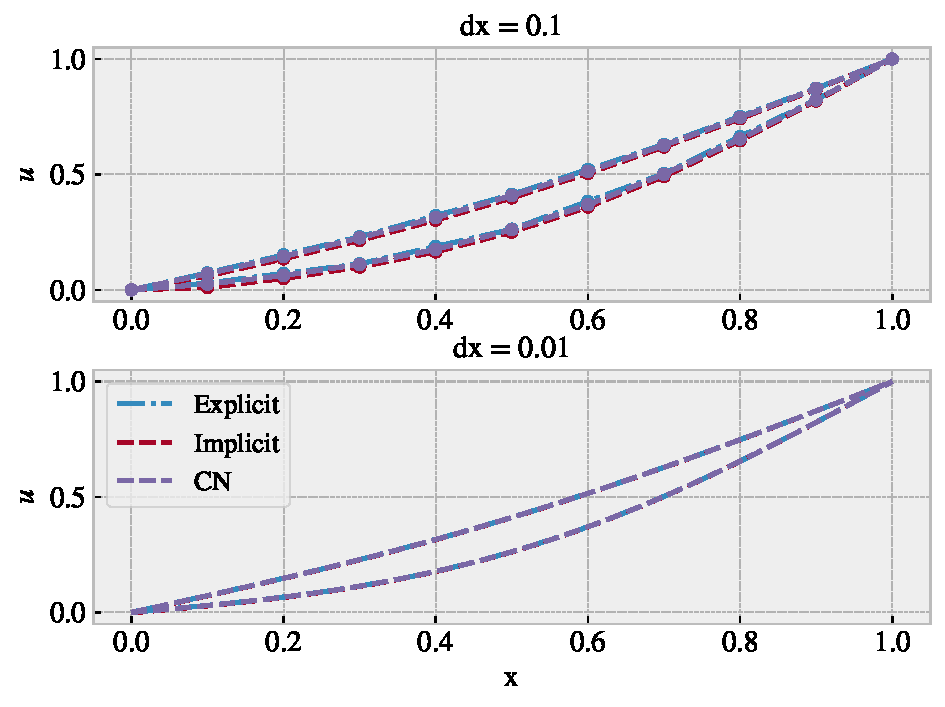
\includegraphics[width=0.5\textwidth]{figures/compare_show.pdf}
%     \caption{...}
%     \label{fig:compare_show.pdf}
% \end{figure}

\onecolumngrid

\begin{figure}[H]
    \centering
    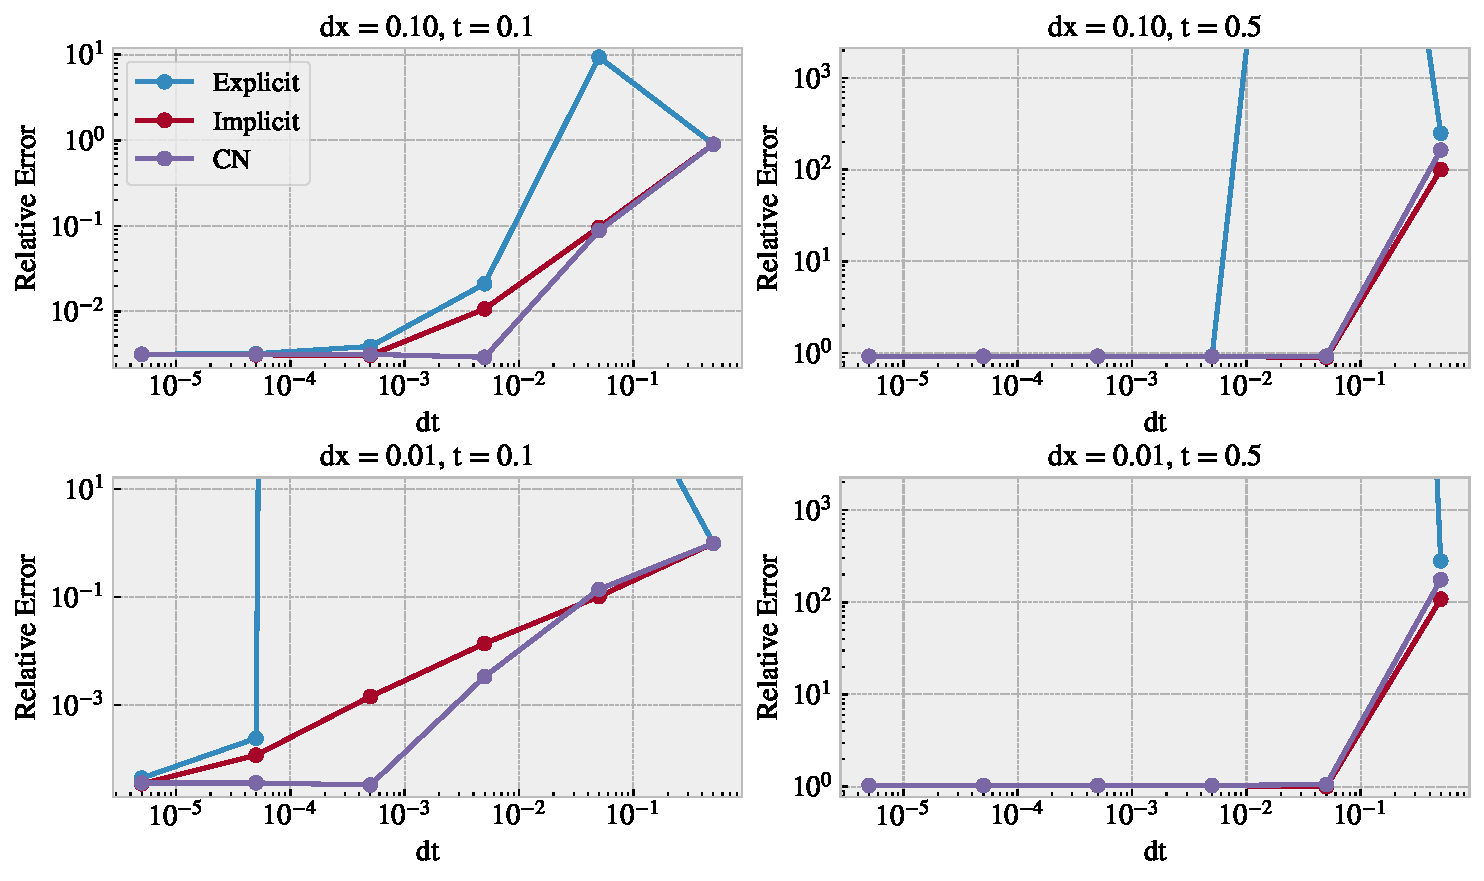
\includegraphics[width=\textwidth]{figures/1D_compare.pdf}
    \caption{The relative error between the numerical and analytical solutions for 1D problem. The relative error is calculated as the average relative error over all points except for $x=0$ since the boundary conditions yields division by zero. We used two different values for spatial step length $dx$ and show the simulation for the time point $t1 = 0.1$ and $t2 = 0.5$ while varying time-step $dt$ on both sides of the stability criteria regarding the explicit method. For $dx = 0.1$ the explicit stability criteria is $dt = 5\times10^{-3}$ and for $dx = 0.01$ it is $dt = 5\times10^{-5}$. Note that the points are plotted on a multiple of 5 times the logarithmic exponential (0.5, 0.05, 0.005 etc.). In three of the cases the graph for the explicit method is cut off because the relative error diverged. For the top right and bottom left plot this resulted in error up to $10^{228}$ and for the bottom right with $dx = 0.001$ and $t = 0.5$ we got overflow.}
    \label{fig:compare_error_dt}
\end{figure}

\twocolumngrid

.
\clearpage
\subsection{Two-dimensional solution to the heat equation }
For the two dimensional problem we used the boundary conditions of zero at all edges and the initial condition state given as $u(t{=}0,x,y) = \sin{(\pi x)}\sin{(\pi y)}$. We used $dx = 0.01$ and $dt = 2.5 \times 10^{-5}$ as dictated by the stability criteria for the explicit method. The solution found by the 2D explicit method is shown in figure \ref{fig:2D_sol}. For the comparison with analytical solution we plotted the relative error between the numerical and analytical solution. For this we excluded the boundary points as this yielded division by zero. The comparison is shown in figure \ref{fig:2D_compare}.


\begin{figure}[H]
    \centering
    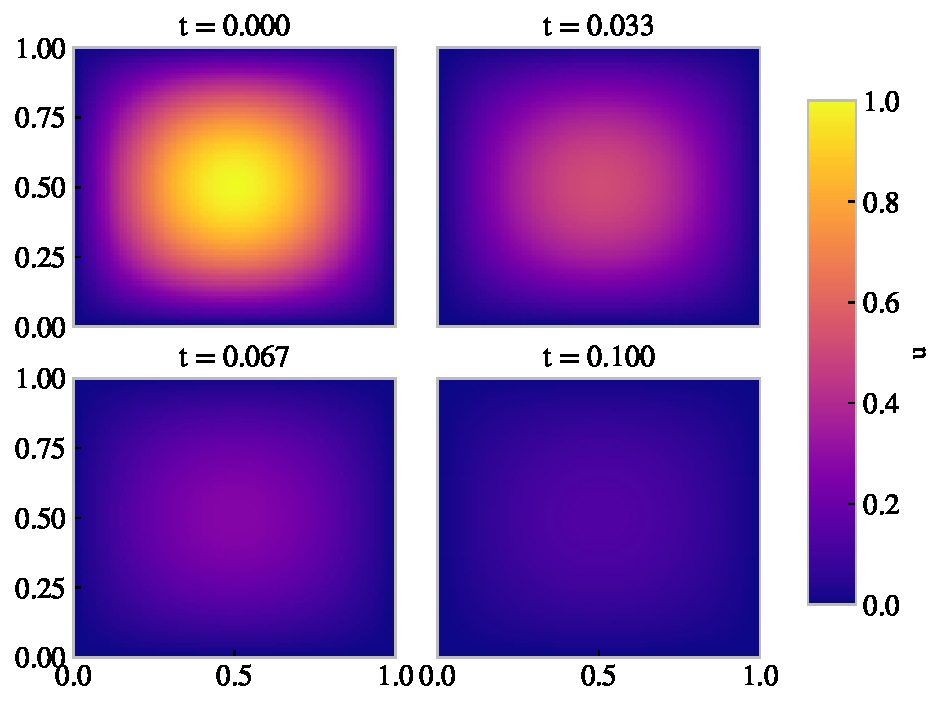
\includegraphics[width=0.5\textwidth]{figures/2D_sol.pdf}
    \caption{Numerical solution to the 2D heat equation defined in section \ref{sec:2D} at four different time points. The boundary are set to zero while the initial condition is given as  $u(t{=}0,x,y) = \sin{(\pi x)}\sin{(\pi y)}$. We used the 2D explicit scheme with $dx = 0.01$ and $dt = 2.5 \times 10^{-5}$ as dictated by the stability criteria.}
    \label{fig:2D_sol}
\end{figure}

\begin{figure}[H]
    \centering
    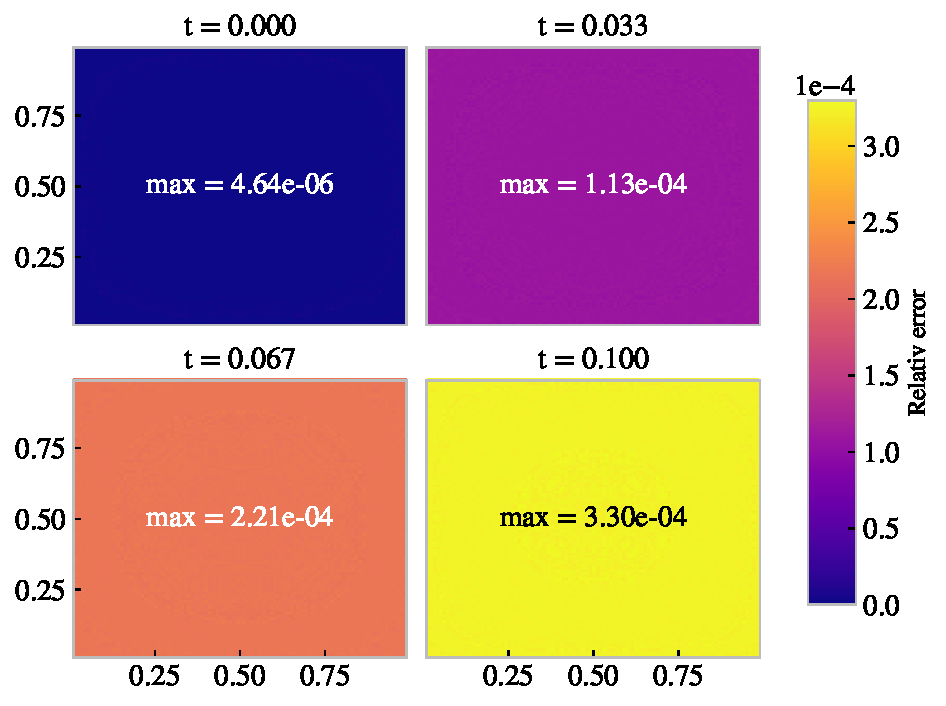
\includegraphics[width=0.5\textwidth]{figures/2D_compare.pdf}
    \caption{The relative error between the numerical solution from figure \ref{fig:2D_sol} and analytical solution from equation \ref{eq:2D_ana} at four different time points. For each time point the maximum relative error is printed on the plots. We excluded the values on the rim since the boundary conditions yields division by zero.}
    \label{fig:2D_compare}
\end{figure}

 Note that we also ran some computations with $dt$ larger than the stability criteria, which gave unstable solutions as expected. We included these in the appendix \ref{sec:2Dunstable}.

\subsection{Temperature distribution in the lithosphere}
\subsubsection{Before radioactive enrichment}
For the study of the temperature distribution in the lithosphere we first studied the case of $Q = 0$ and no radioactive enrichment. The numerical and analytical result are shown in figure \ref{fig:SSBRQ0}. We see that the steady state predicted by the numerical solution matches with the analytical function \ref{eq:SS_ana}. We did a similar computations with the implementation of the piecewise constant function for the natural heat production $Q(z)$ at the different sublayers in the lithosphere. This is shown in figure \ref{fig:SSBR}.

\subsubsection{After radioactive enrichment}
In the next step we studied the actual effect of an radioactive enrichment. We used the steady state obtained from figure \ref{fig:SSBR} after a run time of 1 billion years (Note that this is double as long as shown in figure \ref{fig:SSBR}). We then implemented both models for the radioactive enrichment an simulated the thermal evolution over 1 billion years. The temperature distribution from the model with constant addition to the heat production is shown in figure \ref{fig:AF_Q_constant}, and the second model considering the radioactive decay (according to equation \ref{eq:Q_decay}) is shown in figure \ref{fig:AF_Q_decay}.


\begin{figure}[H]
    \centering
    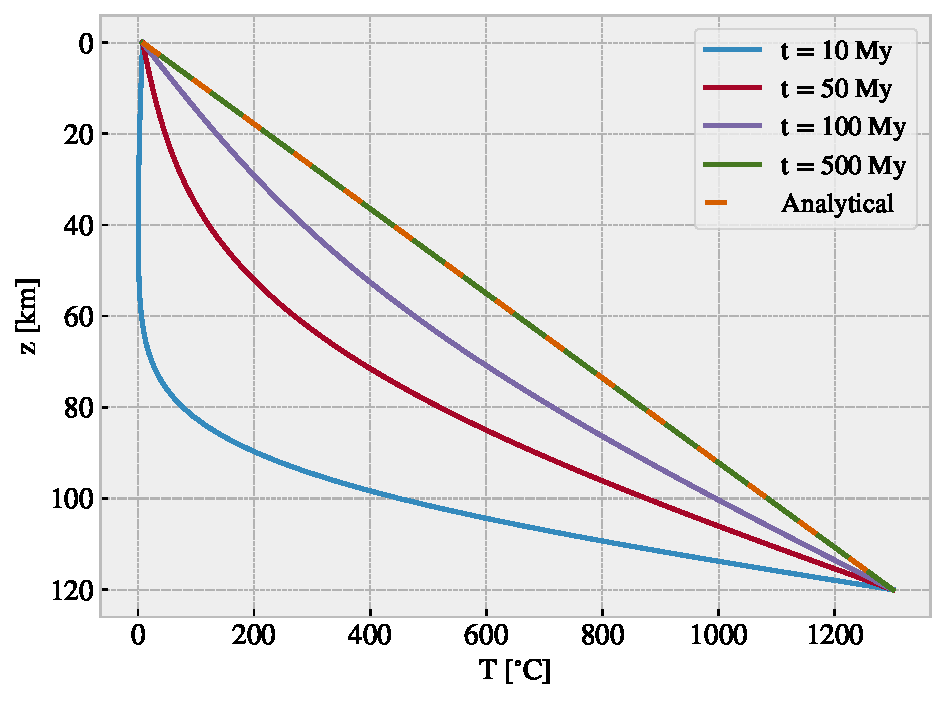
\includegraphics[width=0.5\textwidth]{figures/SteadyState_BRQ0.pdf}
    \caption{The numerical solution for the temperature distribution as a function of depth before radioactive enrichment and with the assumption of no heat production ($Q = 0$). We plotted this together with the analytical solution for the steady state \ref{eq:SS_ana} for similar assumptions. After some time we see an agreement between the numerical and analytical steady state.}
    \label{fig:SSBRQ0}
\end{figure}

\begin{figure}[H]
    \centering
    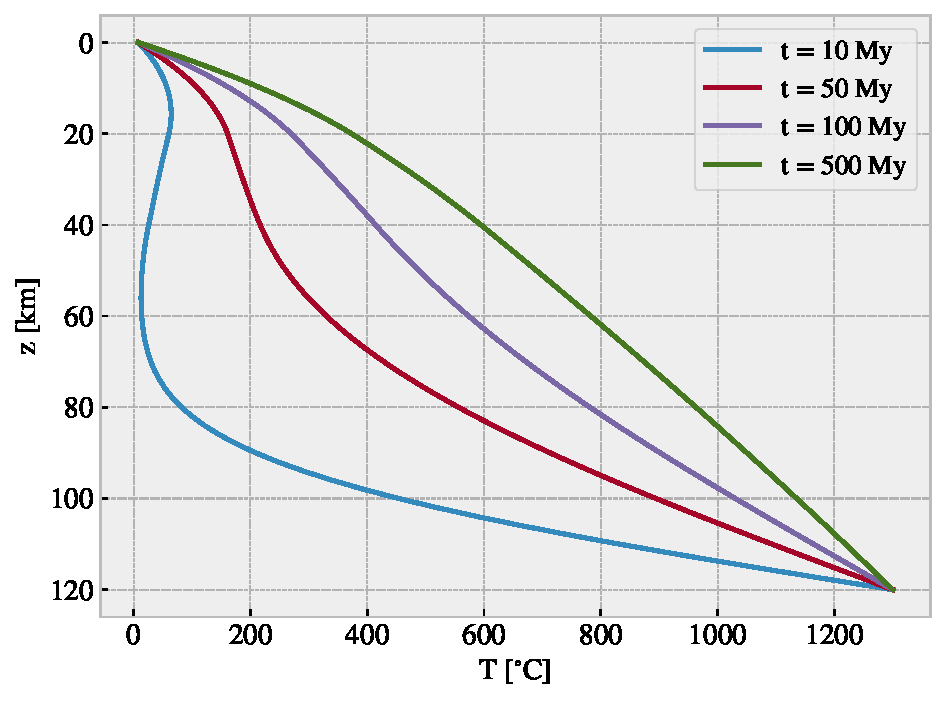
\includegraphics[width=0.5\textwidth]{figures/SteadyState_BR.pdf}
    \caption{The numerical solution for the temperature distribution as a function of depth before radioactive enrichment including the natural heat production $Q(z)$ as a piecewise constant function. We see that the steady state at $t = 500$ million years is not linear.}
    \label{fig:SSBR}
\end{figure}

\begin{figure}[H]
    \centering
    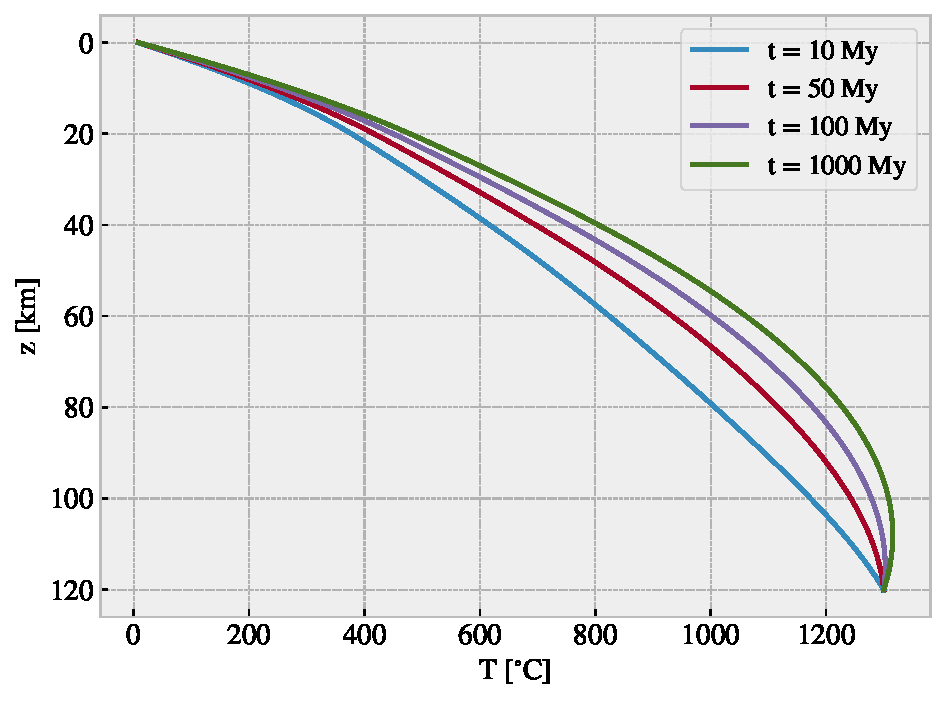
\includegraphics[width=0.5\textwidth]{figures/SteadyState_AR_constant.pdf}
    \caption{The numerical solution for the temperature distribution as a function of depth after radioactive enrichment. In addition to the natural heat production we included at constant value of $Q = 0.5 \mu W/m^3$ for the mantle. We used the steady state distribution obtained in figure \ref{fig:SSBR} as a starting point.}
    \label{fig:AF_Q_constant}
\end{figure}

\hfill \linebreak
\hfill \linebreak
\hfill \linebreak
\hfill \linebreak
\hfill \linebreak
\hfill \linebreak


\begin{figure}[H]
    \centering
    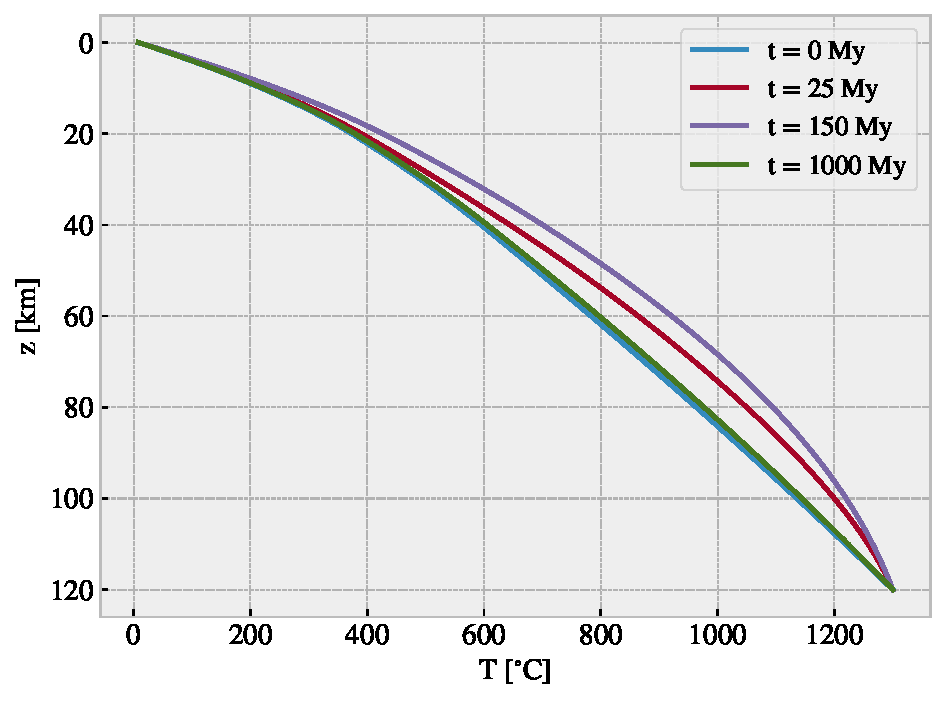
\includegraphics[width=0.5\textwidth]{figures/SteadyState_AR_decay.pdf}
    \caption{The numerical solution for the temperature distribution as a function of depth after radioactive enrichment with decay. In addition to the natural heat production we included a value of $Q = 0.5 \mu W/m^3$ for the mantle which decreased accordingly to the function \ref{eq:Q_decay}. We used the steady state distribution obtained in figure \ref{fig:SSBR} as a starting point.}
    \label{fig:AF_Q_decay}
\end{figure}


From the result in figure \ref{fig:AF_Q_decay} we do some further investigations. We see that the deviation from the original steady state at the beginning gets bigger and then decrease again. To get a clearer picture of this development we plot the point of maximal temperature difference between the beginning steady state and current state as a function of time shown in figure \ref{fig:DeltaT}. In addition we plot the difference in temperature as a function of depth on the last time step corresponding to the distribution at present time shown in figure \ref{fig:DeltaT_Last}. We find that the model predicts a maximal temperature difference of 14.31 $^{\circ}$C at a depth of 66 km. We provided a table (see \ref{tab:max_diff}) of the results from figure \ref{fig:DeltaT_Last} which shows the first few points from a depth-interval which would be considered reachable by humans.


\begin{table}[H]
  \begin{center}
  \caption{Temperature difference for selected depths (corresponding to figure \ref{fig:DeltaT_Last}) for a depth-interval which are somewhat considered directly reachable for humans.}
  \begin{tabular}{|c|c|} \hline
      \textbf{Depth [km]} & \textbf{Temperature difference [$^{\circ}$C]} \\ \hline
      1.0 & 0.280 \\ \hline
      2.0 & 0.559 \\ \hline
      3.0 & 0.838 \\ \hline
      4.0 & 1.118 \\ \hline
      5.0 & 1.397 \\ \hline
      6.0 & 1.676 \\ \hline
      7.1 & 1.955 \\ \hline
      8.1 & 2.234 \\ \hline
      9.1 & 2.512 \\ \hline
      10.1 & 2.790 \\ \hline
      11.1 & 3.068 \\ \hline
      12.1 & 3.346 \\ \hline
  \end{tabular}
  \label{tab:max_diff}
  \end{center}
\end{table}
\begin{figure}[H]
    \centering
    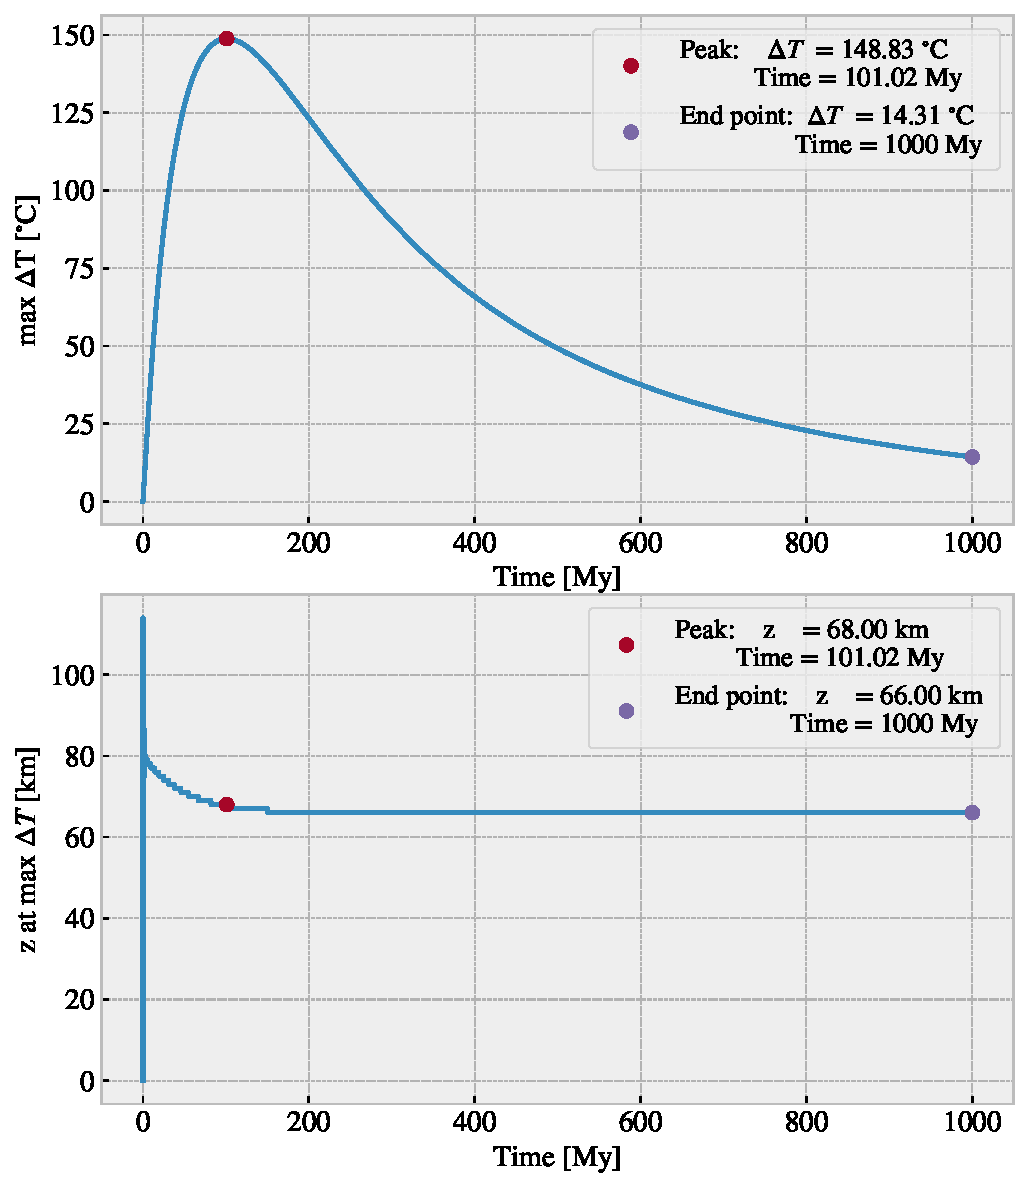
\includegraphics[width=0.5\textwidth]{figures/DeltaT.pdf}
    \caption{The top plot shows the maximum temperature difference $\Delta T$ between the steady state before radioactive enrichment and the temperature distribution after radioactive enrichment as it evolves. The bottom plot shows the corresponding depth $z$ where the maximum $\Delta T$ occurs. In addition we marked the peak value for $\Delta T$ and the corresponding depth $z$, likewise we did with the last time point (end point).}
    \label{fig:DeltaT}
\end{figure}

\begin{figure}[H]
    \centering
    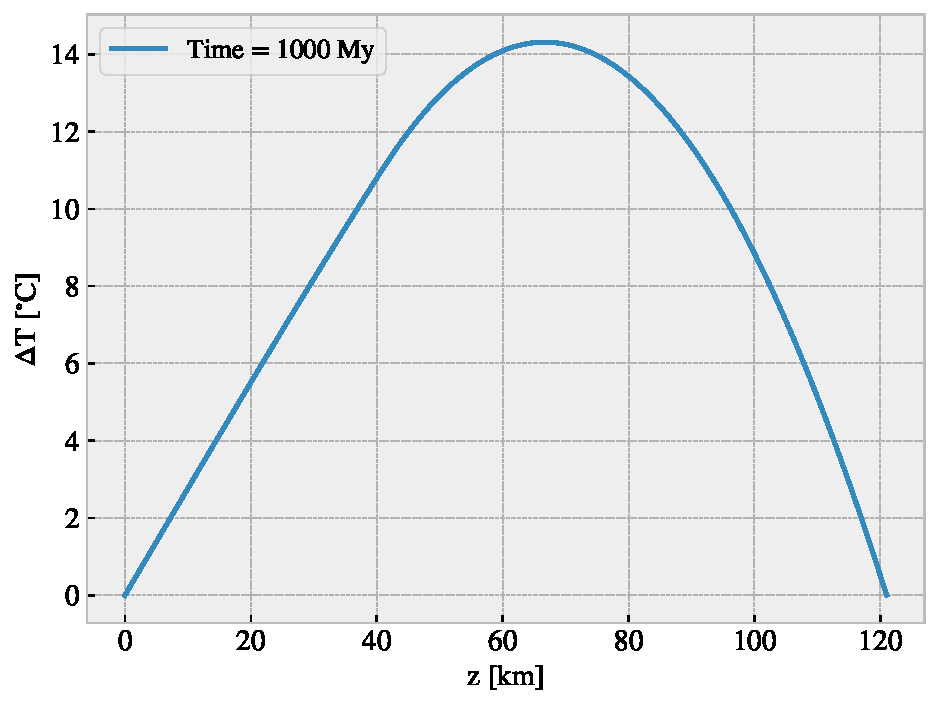
\includegraphics[width=0.5\textwidth]{figures/DeltaT_Last.pdf}
    \caption{Temperature difference as a function of depth 1 Gy after radioactive enrichment. }
    \label{fig:DeltaT_Last}
\end{figure}


\section{Discussion}
\subsection{Comparing the various one-dimensional schemes}
From figure \ref{fig:compare_error_dt} we see that the explicit scheme has the most performance limitations due the stability issue. We see that the relative error diverges when exceeding the stability criteria  $d t \leq \frac{1}{2} d x^2$. For $dx = 0.1$ we have stable values for $dt \leq \num{5e-3}$ and for $dx = 0.01$ we have stable values for $dt \leq  \num{5e-5}$. This match our theoretical expectations. In addition we observed the divergence due to instability to be most extreme for higher $dx$ and higher values of the time point $t$ for which we compared solutions. This also explains why the combination of the highest $dx$ and $t$ gave overflow in all points beyond the stability criteria expect $dt = 0.5$. The reason why the latter point did not overflow is probably because of an insufficient amount of steps to diverge from. The last observation is actually the case for all four combinations of parameters, where we see an somewhat equal error for $dt = 0.5$ when comparing between methods. The difference is most distinct though in the case of higher runtime $t$ and this supports the idea that the number of time steps is simply not sufficient to showcase the \textit{true} behaviour of the method at given parameters. Below the stability criteria we see that the implicit and explicit method perform somewhat equal with an error that goes approximately as $\mathcal{O}(dt)$, which agrees with the theory. This is a qualitative measure since we did not have enough point to justify the use of a linear fit on the log plot. This is due to the fact that the decreasing trend for the relative error was interrupted by a minimum error which seemed to be dictated by a combination of $dx$ and $t$. For $t = 0.1$ it was just above $10^{-3}$ and $10^{-4}$ respectively for $dx = 0.1$ and $dx = 0.01$. For $t = 0.5$ this was about 1 for both choices of $dx$. It is not clear why the latter did not show dependence of $dx$, but it is in general expected to get a limited precision when keeping $dx$ at a constant value. For the CN scheme we also see a convergence towards the same minimum error all though the convergence rate is much faster. Again we did not perform an actual linear fit here, but for some areas it seem to approximately fulfill the theoretical error decrease as $\mathcal{O}(d t^2)$.

% We can tell from the figure that the implicit and CN schemes are always stable. They show similar behavior, but the relative error of the CN scheme decreases faster as $dt$ decreases compared to the implicit scheme. This is because of the truncation error for $dt$ is smaller; $\mathcal{O}(d t^2)$ for the CN scheme comparaed to $\mathcal{O}(d t)$ for the implicit scheme. This is apparent in the plots on the left where the solution is curved, but not in the plots on the right where the solution is linear. Since the solution is linear like the error of the implicit scheme it allows the implicit scheme to perform better as it's error is a good fit for the error of the solution.


\subsection{2D explicit scheme and stability analysis}
In figure \ref{fig:2D_sol} we see that the heat is dissipating quickly, and most of the energy is gone after $t = 0.100$. This is expected from the boundary conditions of zero at the edges and we also se a rather good agreement with the analytical results in figure \ref{fig:2D_compare}. We observe that the maximum relative error increase over time. This can be explained by the simple fact that the error is increased for each timestep. Since the solution will exponentially converge towards zero the relative error will keep increasing even though both the numerical and analytical solutions eventually predicts values practical equal to zero.
 % increases as the difference in energy $u$ decreases. This is expected as the energy difference between the points is smaller, resulting in larger errors due to truncation. For example point $a(x,y) = (0.5,0.5)$ with high energy in the beginning and point $b(x,y) = (0.05,0.05)$ with low energy will have larger relative errors as the energy in $a$ is dissipated throughout the system over time.\\
From the two figures \ref{fig:2D_unstable0.05} and \ref{fig:2D_unstable0.01} in the appendix we see that disregarding the stability condition $dt \geq \frac{h^2}{4}$ also results in unstable solutions as expected for the 2D explicit scheme.

% , where we have done the simulation with a time-step larger than the stability criteria allows $dt \geq \frac{h^2}{4}$. In figure \ref{fig:2D_unstable0.05} we can tell that the $u(x,y)$ values diverge alternatively around time step 34, meaning that the yellow squares reach very high numbers and the blue squares high negative numbers, both approaching overflow. We also saw this in the 1D explicit scheme in figure \ref{fig:compare_error_dt}, which therefore once again verifies the stability issue of the explicit scheme.

% The reason we see yellow squares in the top right corner and not the bottom right corner is because the system is initialized from the bottom left, and as it iterates over x and y it grows more unstable.\\
% In figure \ref{fig:2D_unstable0.01} we see the same behavior as in figure \ref{fig:2D_unstable0.05}, but here the step-size $dx = 0.01$ is smaller. This results in "smaller boxes" with divergent yellow and blue squares. We see here that the solution $u(x,y)$ inhibits some of the periodic traits from the initial conditions $\sin(\pi x)\sin(\pi y)$, and is more unstable around particular parts (at step 36), until almost all the values of $u(x,y)$ diverge (at step 38).

% We can tell from the figures that the instability is dependent on the current step, which is dependant on the value $dt$ in relation to the value $dx$. Around step 34 $u(x,y)$ diverges and we are left with the plots in figure \ref{fig:2D_unstable0.05} and \ref{fig:2D_unstable0.01}.


\subsection{Optimization and timing of the algorithms}
For this project we have not included any timing of the algorithms due to the focus being elsewhere. In order to get a more complete evaluation of the different numerical scheme one should do this. However from a theoretical point of view we see that the explicit scheme should be the fastest algorithm numerically. That is because it only runs a double (or triple in 2D) for-loop that computes the values explicitly, implemented in native $\verb!c++!$. Then comes the implicit scheme, which first initializes Armadillo vectors $a,b,c$ in a for-loop and then performs the Thomas algorithm in another loop. The Crank-Nicolson is the slowest, of course, since it is a combination of both the explicit and the implicit schemes. First it initializes the Armadillo vectors in a for-loop, like the implicit scheme, then computes the values implicitly in another loop, and finally performs the Thomas algorithm in the last loop. The reason we have to initialize the Armadillo vectors for every time-step in the implicit and CN schemes is to save memory, as initializing $(N+2)$ vectors and only using one, would be inefficient use of memory.


\subsection{Temperature distribution in the lithosphere}

\subsubsection{Steady state before radioactive enrichment}
From figure \ref{fig:SSBRQ0} we see a clear match between the numerical and analytical solutions for the temperature distribution with the assumption of $Q = 0$. After implementing the natural heat production in the lithosphere we saw that the temperature increased into a non linear distribution. The difference is most distinct in the upper crust which also corresponds to the layer having the highest heat production. From these observations we find the model acceptable as a base for the natural steady state.

\subsubsection{Temperature distribution after enrichment}
From the numerical computations after radioactive enrichment we find noticeable differences. From the model with a constant addition to the heat production we see a hardly disturbed temperature distribution over time up to 200 $^{\circ}$C. However, this model is also very unrealistic and serves as a top limit for what we can expect. From the more refined model including radioactive decay we see that the max temperature difference peaks around 100 million years after the enrichment. After the full time of a billion years the max difference is reduced to 14.31 $^{\circ}$C at a depth of 66 km. This is a smaller but yet measurable difference. When considering that the largest hole in the world is about 12 km deep it is clear that such measurements at 66 km depths are unrealistic for any geologist to perform. From table \ref{tab:max_diff} we see the more reasonable values to compare with real life measurements, which generally show predicted temperature differences which about one magnitude lower than the max value. It is the beyond the scope of this article to consider the practices of obtaining real life temperature measurements, but given these predictions one have the opportunity to make direct comparisons. If some connection is found this can be used as a supporting argument for the case of determine whether the subduction, and thus the radioactive enrichment, actually happened one billion years ago.

\section{Conclusion}
In this two-part project we have first and foremost addressed the heat equation mathematically for one and two spatial dimension regarding the use of numerical methods. For the one dimensional problem we evaluated the explicit forward Euler method, the implicit backwards Euler method and the implicit Crank-Nicolson method. By investigating the relative errors between the numerical and analytical solutions we found a qualitative agreement with theory; meaning that we saw the explicit and implicit method to yield errors which roughly followd $\mathcal{O}(\Delta t)$, while the Crank-Nicolson method showed a somewhat agreement with $\mathcal{O}(\Delta t^2)$. This is yet to be quantitatively verified for more comprehensive studies. The reason for the vague description of the error trend is due to the presence of a minimum error limit and an instability limit for the explicit method which reduced the number of point of useful data-points. For the former we found that the value of the spatial step $dx$ yielded a limitation to the obtainable precision. Higher values of $dx$ corresponded to a higher minimum error limit, and when extending the time point for which we compared the solution the minimum error limit was raised even further. For the explicit method we verified the instability limit for both one and two dimension. As predicted by theory we found that the explicit method only yielded stable results for
\begin{align*}
  \Delta t \leq \frac{h^2}{2N}
\end{align*}
where $h$ is the constant spatial step-size for all spatial dimensions $N$ and $\Delta t$ is the step length in time. Both the implicit and Crank-Nicolson methods was found to be numerically stable for all values of $h$ and $\Delta t$.
\\
For the two-dimensional problem we only considered the explicit method where we generally found a good agreement with the analytical solution. The relative error was increasing as the solution exponentially converged towards zero, but this is expected for the nature of comparing with relative errors.
\\
In the second part of the project we used the one dimensional explicit scheme to compute the steady state for the temperature distribution in the lithosphere. In the simple case when ignoring the natural heat production due to radioactive decay ($Q = 0$) we found a linear steady state determined by the boundary conditions. This was in agreement with the analytical expression. For the more realistic model including natural heat production as a piecewise constant function we found a non linear distribution as shown in figure \ref{fig:SSBR}. We used this as the base distribution for the case of no radioactive enrichment. When applying the assumed conditions for the radioactive enrichment (considering a decreasing contribution) we found a noticeable deviation from the base distribution. After a time span of 1 billion years we found the resulting maximal temperature difference to be 14.31 $^{\circ}$C at a depth of 66 km. The actual difference in the distribution as a function of depth $z$ is shown in figure \ref{fig:DeltaT_Last} along with predicted differences at reachable depths in table \ref{tab:max_diff}. For the latter we found the temperature difference to be in the range [0.3, 3.3] $^{\circ}$ C for the depth interval [1.0, 12.1] km. If this difference can be verified with real measurements the correspondence can be used to support the theory of the subduction taking place one billion years ago.

\clearpage

\begin{thebibliography}{}
\bibitem{project5} Hoftun F. and Metzsch-Jensen M. (2020), \textit{Project 5 - GitHub repository}, Available at: \url{https://github.com/mikkelme/project5_FYS3150}
\bibitem{project1} Hoftun F. and Metzsch-Jensen M. (2020), \textit{Project 1: Computational Physics - FYS3150}, Available at: \url{https://github.com/mikkelme/Project_1_FYS3150/blob/master/article%20/project1.pdf}
\bibitem{project_description} Univeristy of Oslo, Department of Physics (2020) \textit{Project 5 Diffusion Equation - description}, Available at: \url{http://compphysics.github.io/ComputationalPhysics/doc/Projects/2020/Project5/DiffusionEquation/pdf/DiffusionEquation.pdf}
\bibitem{wiki:PDE} Wikipedia article: Partial differential equation, Available at: \url{https://en.wikipedia.org/wiki/Partial_differential_equation#Introduction}
\bibitem{pdepdf} Hjorth-Jensen M. (2017) \textit{Computational Physics Lectures:Partial differential equations},Available at: \url{http://compphysics.github.io/ComputationalPhysics/doc/pub/pde/pdf/pde-print.pdf}
\bibitem{article} Köhler A., Weidle C., Maupin V (2012) \textit{Crustal and uppermost mantle structure of southern Norway: results from surface wave analysis of ambient seismic noise and earthquake data}, Available at: \url{https://academic.oup.com/gji/article/191/3/1441/563589}

\end{thebibliography}




%\bibliographystyle{plain}

\clearpage
\section*{Appendix}
GitHub repository: \url{https://github.com/mikkelme/project5_FYS3150}

\subsection{Numerical 2D solution with unstable parameters}\label{sec:2Dunstable}
We included some plots of unstable solutions for the 2D problem where we faulty used the 1D stability criteria (twice as big $dt$). The stable solution is shown in figure \ref{fig:2D_sol}.

\begin{figure}[H]
    \centering
    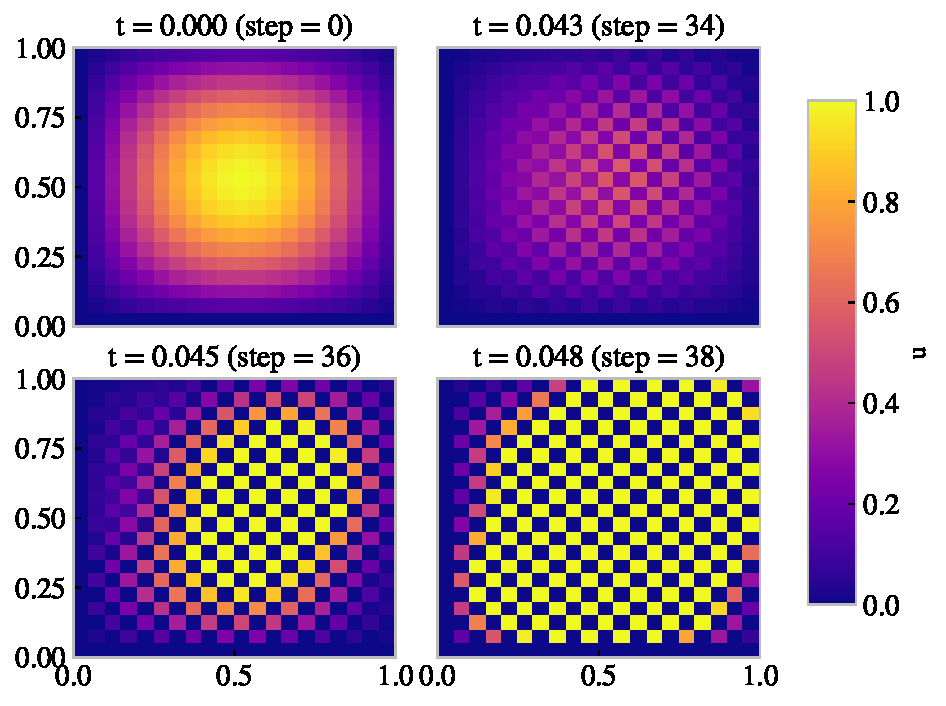
\includegraphics[width=0.5\textwidth]{figures/2D_unstable0.05.pdf}
    \caption{Unstable 2D solution with $dx = 0.05$ and $dt = 2dt_{stable}$ (double the stability criteria). We can see that the solution diverges around time step 34-36 which makes it deteriorate.}
    \label{fig:2D_unstable0.05}
\end{figure}

\begin{figure}[H]
    \centering
    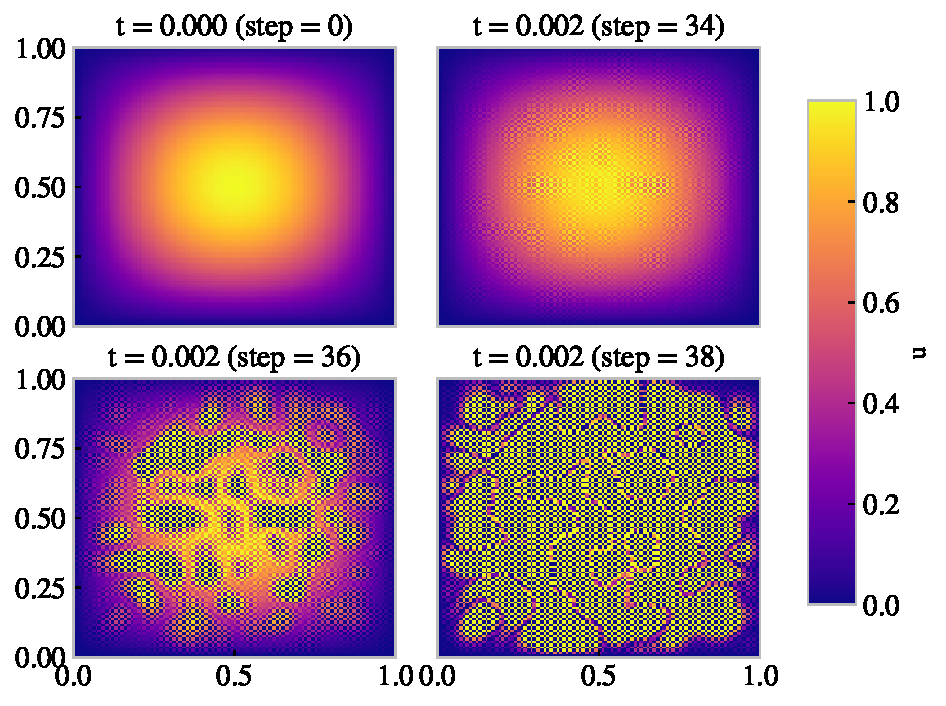
\includegraphics[width=0.5\textwidth]{figures/2D_unstable0.01.pdf}
    \caption{Unstable 2D solution with $dx = 0.01$ and $dt = 2dt_{stable}$ (double the stability criteria). We can see that the solution diverges around time step 34-36 which makes it deteriorate.}
    \label{fig:2D_unstable0.01}
\end{figure}

%Vet at dette er en yalla løsning, men det funker okay...
\hfill \linebreak
\hfill \linebreak
\hfill \linebreak
\hfill \linebreak
\hfill \linebreak
\hfill \linebreak
\hfill \linebreak
\hfill \linebreak
\hfill \linebreak
\hfill \linebreak
\hfill \linebreak
\hfill \linebreak
\hfill \linebreak
\hfill \linebreak
\hfill \linebreak
\hfill \linebreak
\hfill \linebreak
\hfill \linebreak
\hfill \linebreak
\hfill \linebreak
\hfill \linebreak
\hfill \linebreak
\hfill \linebreak
\hfill \linebreak
\hfill \linebreak
\hfill \linebreak
\hfill \linebreak
\hfill \linebreak
\hfill \linebreak
\hfill \linebreak
\hfill \linebreak
\hfill \linebreak
\hfill \linebreak
\hfill \linebreak
\hfill \linebreak
\hfill \linebreak
\hfill \linebreak
\hfill \linebreak
\hfill \linebreak
\hfill \linebreak
\hfill \linebreak
\hfill \linebreak
\hfill \linebreak
\hfill \linebreak
\hfill \linebreak
\hfill \linebreak
\hfill \linebreak
\hfill \linebreak
\hfill \linebreak
\hfill \linebreak
\hfill \linebreak
\hfill \linebreak
\hfill \linebreak
\hfill \linebreak
\hfill \linebreak
\hfill \linebreak
\hfill \linebreak
\hfill \linebreak
\hfill \linebreak
\hfill \linebreak
\hfill \linebreak
\hfill \linebreak
\hfill \linebreak
\hfill \linebreak
\hfill \linebreak
\hfill \linebreak
\hfill \linebreak
\hfill \linebreak


%
% \subsection{Derivation of error in Crank-Nicolson scheme}
% If we have time make the derivation of the error here.
% \\
% To derive the Crank-Nicolson scheme we start with forward Euler scheme and Taylor expand $v(x,t+\Delta t)$ $v(x + \Delta x, t)$, $v(x - \Delta x, t)$:
% \begin{align*}
%     v(x + \Delta x, t) &= v(x,t) + \frac{\partial v(x,t)}{\partial x}\Delta x + \frac{\partial^2 v(x,t)}{2\partial x^2}\Delta x^2 + \mathcal{O}(\Delta x^3) \\
%     v(x - \Delta x, t) &= v(x,t) - \frac{\partial v(x,t)}{\partial x}\Delta x + \frac{\partial^2 v(x,t)}{2\partial x^2}\Delta x^2 + \mathcal{O}(\Delta x^3)\\
%     v(x,t+\Delta t) &= v(x,t) + \frac{\partial v(x,t)}{\partial t}\Delta t + \mathcal{O}(\Delta t^2)
% \end{align*}
% \\
%
%
% \subsection{Trash bin}
% Deleted from explicit scheme:
% \\
% Since we have the boundary conditions $v_{0,t} = v_{L,t} = 0$ we reformulate the algorithm with a matrix-vector formulation:
% \begin{align*}
%     V_{j+1} = \vec{A}V_j
% \end{align*}
% where
% \begin{align*}
%     \vec{A} = \begin{bmatrix}
%                     1-2\alpha & \alpha & 0 & 0 & \cdots \\
%                     \alpha & 1-2\alpha & \alpha & 0 & \cdots \\
%                     \cdots & \cdots & \cdots & \cdots & \cdots \\
%                     \cdots & \cdots & \cdots & \cdots & \alpha \\
%                     0 & 0 & \cdots & \alpha & 1-2\alpha
%     \end{bmatrix}
%     , \qquad V_j =  \begin{bmatrix}
%                         v_{1j} \\
%                         v_{2j} \\
%                         \vdots \\
%                         v_{nj} \\
%                     \end{bmatrix}
% \end{align*}
% We then get
% \begin{align*}
%     V_{j+1} = \vec{A}V_j = \cdots = \vec{A}^{j+1}V_0
% \end{align*}
% where $V_0$ is the initial vector at $t = 0$
% \\
% \\
% \textbf{Ooops} after writing this i saw this in the lecture notes: "In the numerical implementation one should avoid to treat this problem as a matrix vector multiplication since the matrix is triangular and at most three elements in each row are different from zero.". So I do not kow if this is nessecary to include...
% \\
%
% \subsubsection{2D savage shit}
% In order to study a wider variety of systems we will benefit from adding an extra dimension. We will now study $2+1$ dimensions given by 2 spatial dimensions $x$ and $y$ and a time dimension $t$. The diffusion equation then becomes
% \begin{align*}
%     \frac{\partial^2 u(x,y,t)}{\partial x^2} + \frac{\partial^2 u(x,y,t)}{\partial y^2} = \frac{\partial u(x,t)}{\partial t}, \quad t>0 \quad x,y \in [0,L]
% \end{align*}
% We know have more possibilities regarding the choice of boundary conditions. We will look at the simple case where all sides except one is equal to zero and the last is is equal to one. We can express this as:
% \begin{align*}
%       u(0,y,t) &= u(L,y,t) = 0 \\
%       u(x,0,t) &= 0, \quad u(x, L, t) = 1
% \end{align*}
% For the initial condition we use
% \begin{align*}
%      u(x,y,0) &= 0, \qquad 0 < x,y < L \\
% \end{align*}
% We assume to have a $L\times L$ lattice with equally many mesh points $n+2$ in both x- and y-direction. This gives the positional step length $h = L/(n+1)$, and we discretize the variables as
% \begin{align*}
%     &x_i = ih&  &0 \le i \le n+1& \\
%     &y_j = jh&  &0 \le j \le n+1& \\
%     &t_l = l\Delta t& &l \ge 0&
% \end{align*}
% We use the second-order central approximation for the derivation which yields: (Wait... what about trans from u to v?)
% \begin{align*}
%      v_{xx} &= \frac{v(x + h,y, t) - 2v(x,y,t) + v(x -h,y,t)}{h^2} + \mathcal{O}(h^2) \\
%      v_{yy} &= \frac{v(x,y+h, t) - 2v(x,y,t) + v(x,y-h,t)}{h^2} + \mathcal{O}(h^2)
% \end{align*}
% With the new discretized notation we can rewrite this:
% \begin{align*}
%     v_{xx} &= \frac{v_{i+1j}^l - 2v_{ij}^l + v_{i-1j}^l}{h^2} + \mathcal{O}(h^2)\\
%     v_{yy} &=  \frac{v_{ij+1}^l - 2v_{ij}^l + v_{ij-1}^l}{h^2} + \mathcal{O}(h^2)
% \end{align*}
%
% Again we would like to shift the solution such that we obtain zero along all edges and we introduce
% \begin{align*}
%     v(x,y,t) = u(x,y,t) + g(x,y)
% \end{align*}
% analogous to the one dimensional case we can find $g(x,y)$ by inserting this to the diffusion equation and we get
% \begin{align*}
%     \frac{\partial^2g}{dx^2} + \frac{\partial^2g}{dy^2} = 0 \quad \Longrightarrow  \quad \frac{\partial^2g}{dx^2} = - \frac{\partial^2g}{dy^2} = -\lambda^2
% \end{align*}
% where we defined the constant $-\lambda^2$. We assume that the solution to $g$ can be expressed with separation of variables
% \begin{align*}
%     g(x,y) = X(x)Y(y)
% \end{align*}
% for which we get the equation
% \begin{align*}
%     \frac{X''(x)}{X(x)} = - \frac{Y''(y)}{Y(y)} = - \lambda^2
% \end{align*}
% \begin{align*}
%     &X'' + \lambda^2X = 0& &Y'' - \lambda^2Y =0& \\
% \end{align*}
% we get
% \begin{align*}
%     X(x) &= A\sin{(\lambda x)} + B\cos{(\lambda x)} \\
%     Y(y) &= C \sinh{(\lambda y)} + D \cosh{(\lambda y)}
% \end{align*}
% Using the boundary conditions we have $X(0) = 0$, $X(L) = 0$ and $Y(0) = 0$ which gives
% \begin{align*}
%     g(x,y) = B_n\sin{(\frac{n\pi}{L}x)}\sinh{(\frac{n\pi}{L}y)}
% \end{align*}
% Final expression
% \begin{align*}
%     g(x,y) = \sum_{n=1}^\infty B_n\sin{(\frac{n\pi}{L}x)}\sinh{(\frac{n\pi}{L}y)}
% \end{align*}
% We need to find $B_n$. We use
% \begin{align*}
%     g(x,L) = -1 = \sum_{n=1}^\infty B_n\sin{(\frac{n\pi}{L}x)}\sinh{(n\pi)}
% \end{align*}
% Giving
% \begin{align*}
%     B_n \sinh{(n\pi)} &= -\frac{2}{L} \int_0^L \sin{(\frac{n\pi}{L}x)} dx \\
%     &= \frac{2}{n\pi}(\cos{(n\pi)} - 1) \\
%     &= \left\{
%      \begin{array}{@{}l@{\thinspace}l}
%        -\frac{4}{n\pi}  &: \text{n odd}\\
%        0 &: \text{n even}\} \\
%      \end{array}
%    \right.
% \end{align*}
% this gives
% \begin{align*}
%     g(x,y) = \sum_{\text{n odd}} -\frac{4}{n\pi\sinh{(n\pi)}} \sin{(\frac{n\pi}{L}x)} \sinh{(\frac{n\pi}{L}y)}
% \end{align*}
% \\
% \\
% \\
% More trash from 2D analytical
% Use initial conditions to solve for $A_{nm}$.
% \begin{align*}
%     u(x,y,0) = \sin{(x\pi)}y = \sum_{n=1}^\infty \sum_{m=1}^\infty A_{nm}\sin{\left(\frac{n\pi x}{L}\right)} \sin{\left(\frac{m\pi x}{L}\right)}
% \end{align*}
% now get double Fourier series.
% \begin{align*}
%     A_{nm} &= \int_0^L \int_0^L \sin{(x\pi)}\sin{(y\pi)} \sin{\left(\frac{n\pi x}{L}\right)} \sin{\left(\frac{m\pi x}{L}\right)} dxdy \\
%     &=  \int_0^L  \sin{(x\pi)}\sin{\left(\frac{n\pi x}{L}\right)} dx \int_0^L\sin{(y\pi)} \sin{\left(\frac{m\pi x}{L}\right)} dy \\
%     &= \frac{L^2}{\pi^2}\frac{n\sin{(\pi L)}\cos{(n\pi)} - L\cos{(\pi L)}sin{(n\pi)}}{L^2-n^2} \\
%     & \qquad \cdot \frac{m\sin{(\pi L)}\cos{(m\pi)} - L\cos{(\pi L)}sin{(m\pi)}}{L^2-m^2}
% \end{align*}
%

\end{document}

